\documentclass[11pt,a4paper]{article}
\usepackage[utf8]{inputenc}\usepackage[T1]{fontenc}\IfFileExists{italian.ldf}{\usepackage[italian]{babel}}{\usepackage[english]{babel}}\usepackage{amsmath,amssymb,geometry,tikz,graphicx}\geometry{margin=2cm}\usetikzlibrary{arrows.meta,positioning}
\newcommand{\pagina}[1]{\clearpage}
\newcommand{\autfig}[2]{\begin{center}\includegraphics[width=.78\linewidth,height=.32\textheight,keepaspectratio]{automatica_mod_1_tex_assets/fig_#1_#2.png}\end{center}}
\begin{document}\title{Automatica --- Modulo 1}\maketitle
% Pagina originale 1
\section*{Legenda}
\subsection*{1. Introduzione}
\begin{itemize}
\item Cos’è un sistema
\item Orientamento del modello
\item Segnale
\item Riferimento
\item Controllo ad anello aperto
\item Controllo ad anello chiuso
\item Retroazione
\item Schema a blocchi di un sistema di controllo
\item Tassonomia dei sistemi: statico, dinamico, causali, non causali, tempo invarianti, tempo varianti, lineare, non lineare, tempo continuo, tempo discreto
\item PSE
\item Risposta libera
\item Risposta forzata
\end{itemize}
\subsection*{2. SEGNALI CAUSALI}
\begin{itemize}
\item Segnali canonici: impulso di durata finita, delta di Dirac, gradino unitario, rampa unitaria, rampa parabolica
\item Relazione tra segnali canonici
\item Risposta all’impulso
\item Integrale di convoluzione
\end{itemize}
\subsection*{3. TRASFORMATA DI LAPLACE}
\begin{itemize}
\item Proprietà della trasformata
\item Esempi di trasformata
\item Th. valor finale
\item Th. valor iniziale
\item Trasformata della convoluzione
\item Trovare $G(s)$ senza conoscere $g(t)$
\item Proprietà FDT
\item Poli e zeri
\item Rappresentazione della f.d.t.
\item Mappa poli-zeri
\item Velocità del sistema
\item Antitrasformata di Laplace
\item Calcolo di $k_i$
\item Caso di poli complessi coniugati
\item Poli con molteplicità $>1$
\item Calcolare la risposta forzata a $\delta(t)$ conoscendo $G(s)$
\item Th. dei residui
\item Schema a blocchi
\end{itemize}
\subsection*{4. SISTEMI DI PRIMO/SECONDO ORDINE}
\begin{itemize}
\item Sistema del primo ordine
\item Analisi sistema primo ordine privo di zeri
\item Analisi della risposta
\item Tempo di assestamento
\item Tempo di salita
\item Tempo di ritardo
\item Risposta alla rampa
\item Sistemi del primo ordine con uno zero
\item Sistema del secondo ordine
\item Risposta al gradino di un sistema del secondo ordine privo di zeri
\item Inviluppi
\item Massimi e minimi locali
\item Tempo di picco
\item Tempo di salita
\item Tempo di assestamento
\item Luoghi a $\delta$ e $\omega_n$ costante
\item Massima sovraelongazione percentuale
\item Sistemi del secondo ordine con uno zero
\end{itemize}
\subsection*{5. STABILITÀ}
\begin{itemize}
\item Semplicemente stabile
\item Asintoticamente stabile
\item Instabile
\item Classificazione della stabilità in base ai poli di $G(s)$
\item Analisi stabilità sistema ad anello chiuso
\item Lemma di Routh
\item Criterio di Routh-Hurwitz
\item Th. Routh-Hurwitz
\item Stabilità di un sistema con parametri
\end{itemize}
% Pagina originale 2
\pagina{2}
\subsection*{6. ERRORI E DISTURBI}
\begin{itemize}
\item Precisione di sistemi di controllo a regime permanente
\item Errore di posizione
\item Errore di velocità
\item Errore di accelerazione
\item Errore a regime permanente nei sistemi di controllo a retroazione unitaria
\item Reiezione dei disturbi a regime
\item Disturbi sul ramo di retroazione
\item Tecnica di precompensazione dei disturbi
\item Sensibilità alle variazioni parametriche
\end{itemize}
\subsection*{7. LUOGO DELLE RADICI}
\begin{itemize}
\item Regola delle fasi
\item Eq. di taratura
\item Regole di Evans
\end{itemize}
% Pagina originale 3
\pagina{3}
\subsection*{Cos'è un sistema?}
È un complesso di parti collegate tra di loro opportunamente dove è possibile distinguere delle grandezze soggette a variazioni nel tempo (dette variabili).
\subsection*{Orientamento del modello}
Si parla di orientamento di un modello quando avviene la determinazione delle cause e degli effetti di un sistema.
\[\text{cause}\longrightarrow\boxed{\text{Sistema}}\longrightarrow\text{effetti}.\]
Le cause si dicono ingressi $u_i(t)$. Gli effetti si dicono uscite $y_i(t)$. Gli ingressi possono essere manipolabili $u_i(t)$ o non manipolabili (disturbi) $d_i(t)$.
\paragraph{Segnale} È una funzione che esprime il valore di una variabile assunta nel tempo: $f:T\to\mathbb R$.
\paragraph{Riferimento} Esprime il segnale voluto come uscita. È un segnale che esprime l'andamento desiderato di $y(t)$. Se $r_i(t)$ è una costante si parla di setpoint.
\paragraph{Obiettivo del controllo} Progettare un sistema che garantisca che ciascuna uscita $y_i(t)$ insegua il riferimento $r_i(t)$ indipendentemente dai disturbi $d_i(t)$. Ci sono due sottoproblemi sui quali si basa l'introduzione: inseguimento del riferimento; reiezione dei disturbi.

\begin{center}
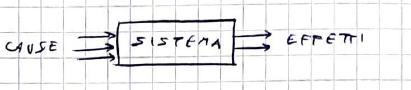
\includegraphics[width=0.75\linewidth]{automatica_mod_1_tex_assets/qa_p03_fig1.png}\par
\end{center}

% Pagina originale 4
\pagina{4}
Idealmente $y(t)=k_c r(t)$ e $e(t)=0$ per ogni $t$. $k_c$ è la costante di proporzionalità, $e(t)$ il segnale dell'errore:
\[e(t):=k_c r(t)-y(t).\]
Se $e(t)=0$ il problema è risolto. Se il riferimento è costante (setpoint) si parla di problema di regolazione; se è variabile si parla di controllo.
\subsection*{Controllo ad anello aperto}
\[r(t)\longrightarrow\boxed{C}\xrightarrow{u(t)}\boxed{S}\xrightarrow{}y(t),\qquad r(t)\longrightarrow\boxed{S\circ C}\longrightarrow y(t).\]
$C$ è il controllore, $S$ il sistema, $S\circ C$ il sistema di controllo. L'anello aperto ha poco controllo del sistema. Viene dato un obiettivo e conoscendo la risposta iniziale possiamo risolvere il problema solo ed esclusivamente in assenza di disturbi.
\subsection*{Controllo ad anello chiuso}
Il riferimento $r$ attraversa il controllore $C$, quindi $u$ entra in $S$ e produce $y$. Il punto di prelievo sull'uscita alimenta il sensore $M$; la sua uscita $\widetilde y$ ritorna al nodo di confronto sul ramo di retroazione (azione).

\begin{center}
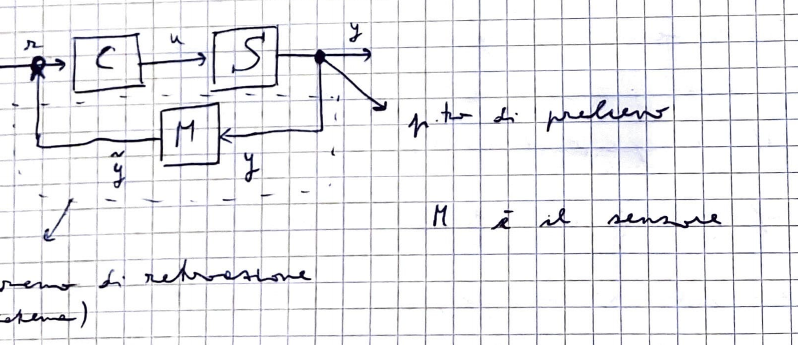
\includegraphics[width=0.75\linewidth]{automatica_mod_1_tex_assets/qa_p04_fig1.png}\par
\end{center}

% Pagina originale 5
\pagina{5}
\subsection*{Retroazione}
Un sistema ad anello chiuso può essere a retroazione negativa (positiva) se interrompendo l'anello in qualsiasi punto e inserendo una perturbazione a valle dell'interruzione, questa ritorna a monte dell'interruzione con segno contrario (stesso segno).
\paragraph{Esempio: retroazione negativa.}
$T=26\,^{\circ}\mathrm C$, $\overline T=25\,^{\circ}\mathrm C$, $e=1\,^{\circ}\mathrm C\Rightarrow u=-1\,^{\circ}\mathrm C$: abbassa di 1.
$T=24\,^{\circ}\mathrm C$, $\overline T=25\,^{\circ}\mathrm C$, $e=-1\,^{\circ}\mathrm C\Rightarrow u=1\,^{\circ}\mathrm C$: alza di 1. Questa è la retroazione negativa dove $u=-e$.
\paragraph{Esempio: retroazione positiva.}
$T=26\,^{\circ}\mathrm C$, $\overline T=25\,^{\circ}\mathrm C$, $e=1\,^{\circ}\mathrm C\Rightarrow u=1\,^{\circ}\mathrm C$: alza di 1.
$T=24\,^{\circ}\mathrm C$, $\overline T=25\,^{\circ}\mathrm C$, $e=-1\,^{\circ}\mathrm C\Rightarrow u=-1\,^{\circ}\mathrm C$: abbassa di 1. Questa è la retroazione positiva dove $u=e$.
Il grafico mostra la ricerca del setpoint $\bar r(t)$, un nuovo disturbo all'istante $\bar t$, l'effetto di disturbi misurabili e l'effetto di disturbi compensati. Non sarebbe possibile senza l'anello chiuso.
La retroazione è insita ovunque. Basta avere un sensore per avere retroazione (è un fatto che venga progettata).

\begin{center}
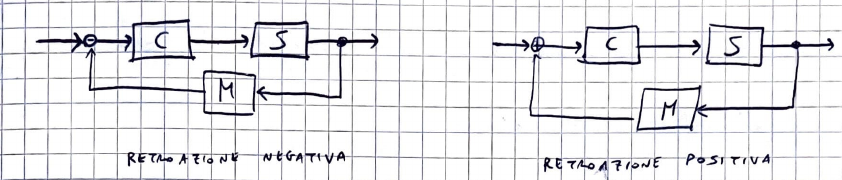
\includegraphics[width=0.75\linewidth]{automatica_mod_1_tex_assets/qa_p05_fig1.png}\par
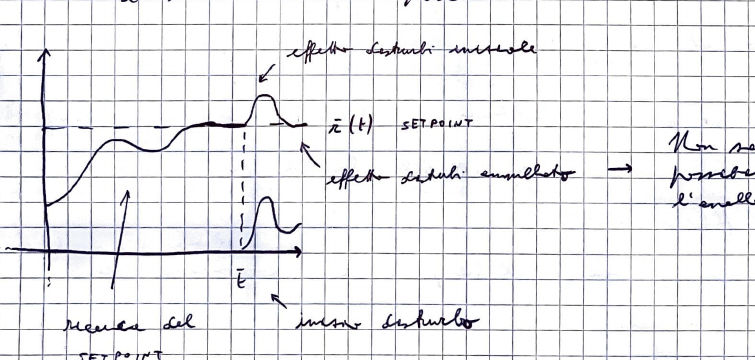
\includegraphics[width=0.75\linewidth]{automatica_mod_1_tex_assets/qa_p05_fig2.png}\par
\end{center}

% Pagina originale 6
\pagina{6}
\subsection*{Schema a blocchi di un sistema di controllo}
\[r(t)\to\boxed{\text{filtro ingresso}}\to\hat r(t)\to\oplus\xrightarrow{e(t)}\boxed C\xrightarrow{u(t)}\boxed A\to\boxed S\to y(t).\]
L'uscita ritorna tramite $M$ al nodo sommatore con segno negativo, come $\hat y(t)$. Il disturbo $d_A$ entra nell'attuatore $A$, $d_S$ nel sistema $S$, e $n(t)$ nel sensore $M$.
$\oplus$ è il nodo sommatore. $\hat y(t)$ è la stima dell'uscita (quella misurata tramite sensori); $\hat r(t)$ è il riferimento scalato; $d_A$ è il disturbo che agisce nell'attuatore; $d_S$ quello che agisce nel sistema; $n(t)$ è il disturbo sulla misura, ``rumore'' (noise).
\[\text{Attuatore}+\text{Sistema}=\text{Impianto (plant)}.\]
\subsection*{Tassonomia dei sistemi}
Statico se la sua uscita al tempo $\bar t$ dipende solo dall'ingresso al tempo $\bar t$. Dinamico se non è statico. Sono dinamici i sistemi modellabili tramite relazioni integro-differenziali. Per conoscere l'uscita al tempo $\bar t$ devi conoscere le condizioni iniziali.
Causali se l'uscita al tempo $\bar t$ non dipende dai valori futuri dell'ingresso (c'è un nesso di causa-effetto). Non causali se non sono causali.

\begin{center}
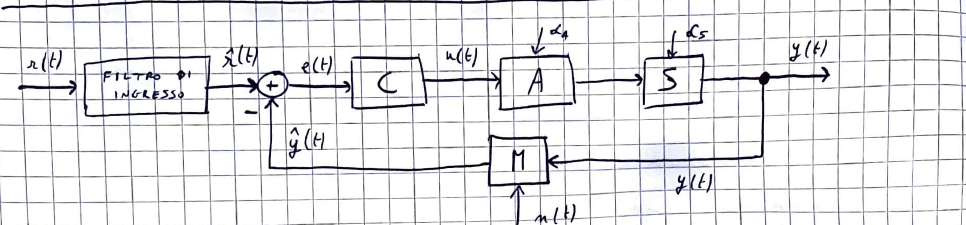
\includegraphics[width=0.75\linewidth]{automatica_mod_1_tex_assets/qa_p06_fig1.png}\par
\end{center}

% Pagina originale 7
\pagina{7}
Tempo invarianti se e solo se l'uscita prodotta dal sistema in risposta a un ingresso $\bar u$ ritardato di $\tau>0$ secondi è pari all'uscita senza ritardo dell'ingresso $\bar u$. Indica che il sistema non dipende dal momento in cui viene utilizzato e/o dalle condizioni o eventi precedenti.
Tempo variante se non è tempo invariante. Lineare se vale il PSE; non lineare se non vale il PSE. Tempo continuo se $t$ varia con continuità ($t\in\mathbb R$); tempo discreto se $t$ varia in un insieme con relazione $\bar t=kt_0$, $k\in\mathbb N$ ($t_0$ tempo di campionamento).
\subsection*{Principio di sovrapposizione degli effetti (PSE)}
Applico separatamente $u_i(t)$ ingressi e produco $y_i(t)$ uscite. Date $m$ costanti $k_i$, applicando
\[u(t)=\sum_{i=1}^{m}k_i u_i(t),\qquad y(t)=\sum_{i=1}^{m}k_i y_i(t).\]
Vale solo per sistemi lineari.
\subsection*{Risposte libera e forzata}
La soluzione di un'equazione differenziale $y(t)$ si può scrivere in due contributi:
\[y(t)=y_l(t)+y_f(t).\]
$y_l(t)$ è la risposta libera ($u(t)=0$); $y_f(t)$ è la risposta forzata (condizioni iniziali nulle); $y$ è la risposta completa.
% Pagina originale 8
\pagina{8}
\subsection*{Segnale causale e segnali canonici}
È causale se $x(t)=0$ per ogni $t<0$.
Impulso di durata finita:
\[P_\tau(t)=\begin{cases}1/\tau&0\le t\le\tau,\\0&\text{altrove},\end{cases}\qquad \int_{-\infty}^{\infty}P_\tau(t)\,dt=1.\]
Delta di Dirac: $\delta(t)\triangleq\lim_{\tau\to0}P_\tau(t)$; rappresentazione intuitiva $\delta(t)=\infty$ per $t=0$, $0$ per $t\ne0$. Proprietà:
\[\forall\varepsilon>0:\ \int_{-\varepsilon}^{\varepsilon}\delta(t)\,dt=1\quad(\text{massa}),\qquad \int_{-\infty}^{\infty}\delta(t-\tau)f(t)\,dt=f(\tau)\quad(\text{campionamento}).\]
Dimostrazione: $\delta(t-\tau)f(t)=\delta(t-\tau)f(\tau)$; quindi l'integrale è $f(\tau)\int_{-\infty}^{\infty}\delta(t-\tau)dt=f(\tau)$.
Gradino unitario:
\[1(t)=\begin{cases}1&t\ge0,\\0&t<0.\end{cases}\]
Qualsiasi ingresso costante a tratti può essere espresso come combinazione lineare di segnali a gradino opportunamente ritardati nel tempo.

\begin{center}
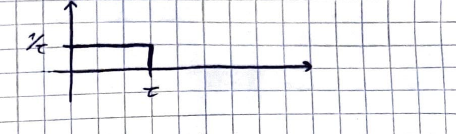
\includegraphics[width=0.75\linewidth]{automatica_mod_1_tex_assets/qa_p08_fig1.png}\par
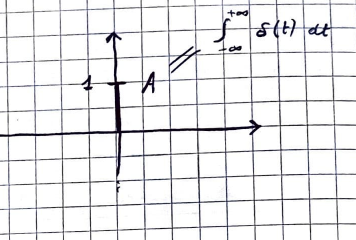
\includegraphics[width=0.75\linewidth]{automatica_mod_1_tex_assets/qa_p08_fig2.png}\par
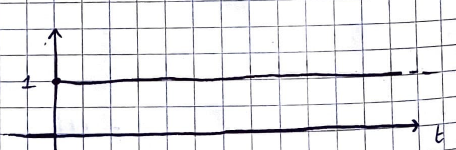
\includegraphics[width=0.75\linewidth]{automatica_mod_1_tex_assets/qa_p08_fig3.png}\par
\end{center}

% Pagina originale 9
\pagina{9}
\[P_\tau(t)=\frac1\tau1(t)-\frac1\tau1(t-\tau).\]
Rampa unitaria: $f(t)=t$ per $t\ge0$, $0$ per $t<0$, ossia $f(t)=t1(t)$. Rampa parabolica: $f(t)=t^2/2$ per $t\ge0$, $0$ per $t<0$, ossia $f(t)=\frac{t^2}{2}1(t)$.
\subsection*{Relazioni tra segnali canonici}
\[\delta\xrightarrow{\int}1(t)\xrightarrow{\int}t1(t)\xrightarrow{\int}\frac{t^2}{2}1(t).\]
Per $\bar t>0$:
\[\int_{-\infty}^{\bar t}\delta(t)dt=\int_{-\infty}^{0^-}\delta(t)dt+\int_{0^-}^{0^+}\delta(t)dt+\int_{0^+}^{\bar t}\delta(t)dt=1.\]
Per $\bar t<0$ l'integrale è zero. Dunque
\[\int_{-\infty}^{\bar t}\delta(t)dt=1(\bar t),\quad\int_{-\infty}^{\bar t}1(t)dt=\bar t1(\bar t),\quad\int_{-\infty}^{\bar t}t1(t)dt=\frac{\bar t^2}{2}1(\bar t).\]
\[\frac d{dt}\left[\frac{t^2}2 1(t)\right]=t1(t),\qquad\frac d{dt}[t1(t)]=1(t),\qquad\frac d{dt}1(t)\triangleq\delta(t).\]
La derivata generalizzata di $1(t)$ è $\delta(t)$.

\begin{center}
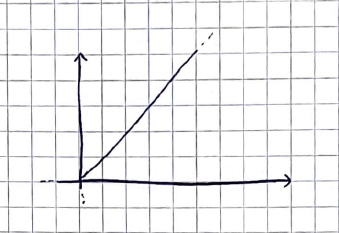
\includegraphics[width=0.75\linewidth]{automatica_mod_1_tex_assets/qa_p09_fig1.png}\par
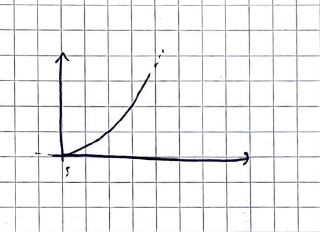
\includegraphics[width=0.75\linewidth]{automatica_mod_1_tex_assets/qa_p09_fig2.png}\par
\end{center}

\[\frac{d}{dt}\left[\frac{t^2}{2}1(t)\right]=
\begin{cases}\frac{d}{dt}\frac{t^2}{2}&t\ge0,\\\frac{d}{dt}0&t<0\end{cases}
=\begin{cases}t&t\ge0,\\0&t<0\end{cases}=t1(t).\]

% Pagina originale 10
\pagina{10}
\subsection*{Risposta all'impulso}
$g(t)$ è la risposta forzata di un sistema LTI a $\delta(t)$; è chiamata risposta all'impulso.
\subsection*{Integrale di convoluzione}
Approssimo $u(t)$ con un segnale costante a tratti espresso come somma di impulsi:
\begin{align*}
u(t)&\simeq\sum_i P_{\Delta\tau}(t-\tau_i)u(\tau_i)\Delta\tau\\
&=\sum_i\begin{cases}\frac1{\Delta\tau}u(\tau_i)\Delta\tau&t\in[\tau_i,\tau_{i+1}],\\0&\text{altrove}\end{cases}\\
&=\sum_{i=0}^{m-1}u(\tau_i)[1(t-\tau_i)-1(t-\tau_{i+1})].
\end{align*}
Se $\Delta\tau\to0$, la differenza dei gradini tende a $\delta(t-\tau_i)\Delta\tau$. Se $g(t)$ è la risposta a $\delta(t)$, allora $\Delta\tau g(t-\tau_i)$ è la risposta a $\Delta\tau\delta(t-\tau_i)$. Per il PSE:
\[y_f(t)\simeq\sum_{i=0}^{m-1}g(t-\tau_i)u(\tau_i)\Delta\tau.\]
Visto che $\Delta\tau\to0\Rightarrow m\to\infty$, la somma diventa un integrale:
\[y_f(t)=\int_0^\infty u(\tau)g(t-\tau)d\tau=u(t)*g(t)=g(t)*u(t).\]
L'asterisco è l'operatore convoluzione. Separando l'integrale a $t$, la parte da $t$ a $\infty$ è nulla poiché $g(x)=0$ per $x<0$.

\begin{center}
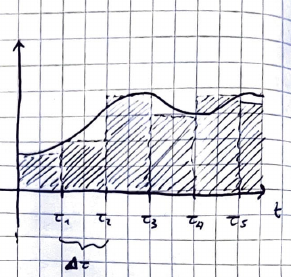
\includegraphics[width=0.75\linewidth]{automatica_mod_1_tex_assets/qa_p10_fig1.png}\par
\end{center}

\[u(t)=\sum_{i=0}^{m-1}u(\tau_i)[1(t-\tau_i)-1(t-\tau_{i+1})]
\xrightarrow{\Delta\tau\to0}\sum_{i=0}^{m-1}u(\tau_i)\delta(t-\tau_i)\Delta\tau.\]
\[y_f(t)=\int_0^t u(\tau)g(t-\tau)d\tau+
\underbrace{\int_t^\infty u(\tau)g(t-\tau)d\tau}_{0:\ g(x)=0\text{ per }x<0}.\]
\emph{Nota di trascrizione (p.~10): nella riga manoscritta con $1/\Delta\tau$ il membro destro contiene anche $\Delta\tau$; la riga successiva mostra la decomposizione degli impulsi. Si conserva qui la decomposizione leggibile.}

% Pagina originale 11
\pagina{11}
La convoluzione corrisponde al prodotto tra segnali:
\[y_f(t)=\int_0^t u(\tau)g(t-\tau)d\tau.\]
Il disegno rappresenta lo scorrimento del segnale $g(t-\tau)$ rispetto a $u(\tau)$ e l'area del loro prodotto.
\subsection*{Trasformata di Laplace}
L'operatore ``trasformata unilaterale di Laplace'' è una trasformazione che associa ad una funzione causale $f:\mathbb R\to\mathbb R$ una funzione $F(s):\mathbb C\to\mathbb C$:
\[\mathcal L\{f(t)\}=F(s)\triangleq\int_{0^-}^{\infty}e^{-st}f(t)dt,\qquad s=\sigma+j\omega.\]
Si richiede $e^{-st}\to0$ quando $t\to\infty$.
\[\mathcal L\{\delta(t)\}=\int_{0^-}^{\infty}e^{-st}\delta(t)dt=e^{-s0}=1\]
sfruttando la proprietà del campionamento. $\mathcal L\{\delta(t)\}=\Delta(s)=1$.
\[\mathcal L\{1(t)\}=\int_0^\infty e^{-st}dt=-\frac1s[e^{-st}]_0^\infty=-\frac1s(0-1)=\frac1s\]
solo se $\operatorname{Re}s>0$. Infatti $|e^{-st}|=|e^{-\sigma t}||e^{-j\omega t}|=|e^{-\sigma t}|$, il cui limite è $0$ se $\sigma>0$, $1$ se $\sigma=0$, $\infty$ se $\sigma<0$.

\begin{center}
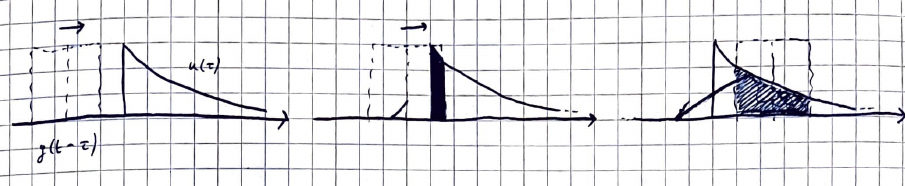
\includegraphics[width=0.75\linewidth]{automatica_mod_1_tex_assets/qa_p11_fig1.png}\par
\end{center}

% Pagina originale 12
\pagina{12}
\subsection*{Proprietà della trasformata}
\begin{enumerate}
\item Linearità:
\[\mathcal L\{\alpha f_1(t)+\beta f_2(t)\}=\alpha\mathcal L\{f_1(t)\}+\beta\mathcal L\{f_2(t)\}.\]
Dimostrazione: dalla linearità dell'integrale.
\item $\mathcal L\{f(t-\tau)\}=e^{-s\tau}\mathcal L\{f(t)\}$. Ponendo $T=t-\tau$:
\[\int_{0^-}^\infty f(t-\tau)e^{-st}dt=\int_{0^- -\tau}^{\infty}f(T)e^{-s(T+\tau)}dT=e^{-s\tau}\int_0^\infty f(T)e^{-sT}dT.\]
\item $\mathcal L\{f(t)e^{at}\}=F(s-a)$. Infatti $\int_{0^-}^{\infty}f(t)e^{at}e^{-st}dt=\int_{0^-}^{\infty}f(t)e^{-(s-a)t}dt$.
\item $\mathcal L\{t^m f(t)\}=(-1)^m\frac{d^mF(s)}{ds^m}$. Per $m=1$:
\[\frac d{ds}F(s)=\int_{0^-}^{\infty}\frac d{ds}e^{-st}f(t)dt=\int_{0^-}^{\infty}(-t)e^{-st}f(t)dt=-\mathcal L\{tf(t)\}.\]
Si continua per induzione.
\item $\mathcal L\{f^{(m)}(t)\}=s^mF(s)-s^{m-1}f(0)-\cdots-f^{(m-1)}(0)$. Se le condizioni iniziali sono tutte nulle: $\mathcal L\{f^{(m)}(t)\}=s^mF(s)$.
\item $\mathcal L\{\int_0^t f(\tau)d\tau\}=\frac1sF(s)$.
\end{enumerate}
\paragraph{Passaggi della dimostrazione della proprietà 3.}
Ponendo $z=s-a$:
\[\int_{0^-}^{\infty}f(t)e^{-(s-a)t}dt
=\int_{0^-}^{\infty}f(t)e^{-zt}dt=F(z)=F(s-a).\]
\paragraph{Passaggi della proprietà 4.}
\[\frac d{ds}F(s)=\frac d{ds}\int_{0^-}^{\infty}e^{-st}f(t)dt
=\int_{0^-}^{\infty}\frac d{ds}(e^{-st})f(t)dt
=\int_{0^-}^{\infty}f(t)(-t)e^{-st}dt.\]

% Pagina originale 13
\pagina{13}
\subsection*{Esempi di trasformate}
\begin{align*}
\mathcal L\{e^{-at}1(t)\}&=\left.\frac1s\right|_{s+a}=\frac1{s+a},\\
\mathcal L\{t1(t)\}&=-\frac d{ds}\frac1s=\frac1{s^2},\\
\mathcal L\{\tfrac{t^2}2 1(t)\}&=\frac12\frac{d^2}{ds^2}\frac1s=\frac1{s^3},\\
\mathcal L\{\sin(\omega t)1(t)\}&=\frac1{2j}\left(\frac1{s-j\omega}-\frac1{s+j\omega}\right)=\frac\omega{s^2+\omega^2},\\
\mathcal L\{\cos(\omega t)1(t)\}&=\frac12\left(\frac1{s-j\omega}+\frac1{s+j\omega}\right)=\frac s{s^2+\omega^2}.
\end{align*}
Si usano $\sin(\omega t)=(e^{j\omega t}-e^{-j\omega t})/(2j)$ e $\cos(\omega t)=(e^{j\omega t}+e^{-j\omega t})/2$.
\subsection*{Teorema del valor finale}
Sia $f(t)$ un segnale causale al quale è associato $F(s)=\mathcal L\{f(t)\}$. Se esiste $\lim_{t\to\infty}f(t)\in\mathbb R$, allora
\[\lim_{t\to\infty}f(t)=\lim_{s\to0}sF(s),\]
e $sF(s)$ ha tutte le singolarità nel semipiano sinistro ($\operatorname{Re}s<0$). Le singolarità sono i valori di $s$ dove $sF(s)\to\infty$, cioè i poli.
\subsection*{Teorema del valor iniziale}
\[\lim_{t\to0}f(t)=\lim_{s\to\infty}sF(s).\]
\paragraph{Passaggi delle trasformate.}
\begin{align*}
\mathcal L\{t1(t)\}&=\frac d{ds}\frac1s(-1)^1=-\left(-\frac1{s^2}\right)=\frac1{s^2},\\
\mathcal L\{\tfrac{t^2}{2}1(t)\}&=\frac12\frac{d^2}{ds^2}\frac1s(-1)^2
=\frac12\frac d{ds}\left(-\frac1{s^2}\right)=\frac12\frac2{s^3}=\frac1{s^3},\\
\mathcal L\{\sin(\omega t)1(t)\}&=\mathcal L\{\tfrac{e^{j\omega t}-e^{-j\omega t}}{2j}1(t)\}\\
&=\tfrac1{2j}\mathcal L\{e^{j\omega t}1(t)\}-\tfrac1{2j}\mathcal L\{e^{-j\omega t}1(t)\}\\
&=\tfrac1{2j}\tfrac1{s-j\omega}-\tfrac1{2j}\tfrac1{s+j\omega}
=\tfrac1{2j}\tfrac{2j\omega}{s^2+\omega^2},\\
\mathcal L\{\cos(\omega t)1(t)\}&=\mathcal L\{\tfrac{e^{j\omega t}+e^{-j\omega t}}2 1(t)\}\\
&=\tfrac12\mathcal L\{e^{j\omega t}1(t)\}+\tfrac12\mathcal L\{e^{-j\omega t}1(t)\}
=\tfrac12\tfrac{2s}{s^2+\omega^2}.
\end{align*}

% Pagina originale 14
\pagina{14}
\subsection*{Trasformata della convoluzione}
\[h(t)=f_1(t)*f_2(t)=\int_{-\infty}^{\infty}f_1(t-\tau)f_2(\tau)d\tau=\int_{0^-}^{t}f_1(t-\tau)f_2(\tau)d\tau.\]
\[\mathcal L\{h(t)\}=\int_0^\infty\left[\int_0^t f_1(t-\tau)f_2(\tau)d\tau\right]e^{-st}dt=F_1(s)F_2(s).\]
Quindi $\mathcal L\{f_1*f_2\}=\mathcal L\{f_1\}\mathcal L\{f_2\}$. So che $y_f(t)=g(t)*u(t)$, perciò $Y_f(s)=G(s)U(s)$, rappresentato dal blocco $U(s)\to\boxed{G(s)}\to Y(s)$.
\subsection*{Trovare $G(s)$ senza conoscere $g(t)$}
1) $G(s)=Y_f(s)/U(s)$. 2) Conoscendo il modello matematico del sistema:
\[\sum_{i=0}^{n}a_iD^iy(t)=\sum_{i=0}^{m}b_iD^iu(t),\qquad n\ge m,\quad a_i,b_i\in\mathbb R.\]
Applico Laplace e la linearità:
\[\sum_{i=0}^{n}a_i\left(s^iY(s)-\sum_{j=0}^{i-1}y^{(i-j-1)}(0)s^j\right)=\sum_{i=0}^{m}b_i s^iU(s),\]
con condizioni iniziali dell'ingresso nulle. Riordinando:
\[\underbrace{\sum_{i=0}^{n}a_i s^i}_{a(s)}Y(s)-\underbrace{\sum_{i=0}^{n}\sum_{j=0}^{i-1}a_i y^{(i-j-1)}(0)s^j}_{c(s)}=\underbrace{\sum_{i=0}^{m}b_i s^i}_{b(s)}U(s).\]
$a(s)$ è di grado $n$, $c(s)$ di grado $n-1$, $b(s)$ di grado $m$.
\paragraph{Passaggio mediante la linearità.}
\[\mathcal L\left\{\sum_{i=0}^n a_iD^iy(t)\right\}
=\mathcal L\left\{\sum_{i=0}^m b_iD^iu(t)\right\}
\quad\Longrightarrow\quad
\sum_{i=0}^n a_i\mathcal L\{D^iy(t)\}
=\sum_{i=0}^m b_i\mathcal L\{D^iu(t)\}.\]
$n\ge m$: sistema causale.

% Pagina originale 15
\pagina{15}
\[a(s)Y(s)-c(s)=b(s)U(s)\Rightarrow Y(s)=\underbrace{\frac{b(s)}{a(s)}U(s)}_{Y_f(s)}+\underbrace{\frac{c(s)}{a(s)}}_{Y_l(s)}.\]
\[G(s)=\frac{b(s)}{a(s)}=\frac{b_ms^m+b_{m-1}s^{m-1}+\cdots+b_1s+b_0}{a_ns^n+a_{n-1}s^{n-1}+\cdots+a_1s+a_0}.\]
È la funzione di trasferimento. Esempio:
\[2\frac{d^3y}{dt^3}+3\frac{d^2y}{dt^2}+2\frac{dy}{dt}-y=3\frac{du}{dt}-5u,\qquad G(s)=\frac{3s-5}{2s^3+3s^2+2s-1}.\]
\subsection*{Proprietà FDT}
È una funzione razionale fratta; $G(s)=Y_f(s)/U(s)=b(s)/a(s)$; $G(s)=\mathcal L\{g(t)\}$, trasformata della risposta all'impulso.
Con $m=\deg b$, $n=\deg a$, può essere propria ($m=n$), strettamente propria ($m<n$), impropria ($m>n$, non causale quindi). Esempi: $(s^2+2s+2)/(s^2+3)$, $(s-1)/(s^4+2)$, $s^2/(s-1)$ rispettivamente.
\subsection*{Poli e zeri}
Poli: tutte le $n$ radici complesse di $a(s)$ dove $|G(s)|\to\infty$. Zeri: tutte le $m$ radici complesse di $b(s)$ dove $G(s)=0$.

\begin{center}
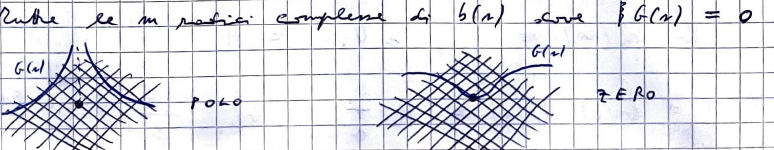
\includegraphics[width=0.75\linewidth]{automatica_mod_1_tex_assets/qa_p15_fig1.png}\par
\end{center}

% Pagina originale 16
\pagina{16}
\subsection*{Rappresentazione della FDT}
\[G(s)=\frac{\sum b_i s^i}{\sum a_i s^i}=\frac{b_m}{a_n}\frac{\prod(s-z_i)}{\prod(s-p_i)}=k_0\frac{\prod(s-z_i)}{\prod(s-p_i)},\quad k_0=\frac{b_m}{a_n}.\]
\subsection*{Mappa poli-zeri}
Per $G(s)=(s+3)/[(s-1)(s+1)(s+2)^2]$, zero in $-3$ (cerchio), poli in $-2$ (doppio), $-1$, $1$ (croci). Il grafico esprime $G(s)/k_0$ e non $G(s)$.
\[G(s)=k_0\frac{\prod(-z_i)\prod(1-s/z_i)}{\prod(-p_i)\prod(1-s/p_i)}=k_1\frac{\prod(1+\tau_{z_i}s)}{\prod(1+\tau_{p_i}s)},\]
\[k_1=k_0\frac{\prod(-z_i)}{\prod(-p_i)},\quad \tau_{z_i}=-\frac1{z_i},\quad\tau_{p_i}=-\frac1{p_i}.\]
$k_1$ è il guadagno statico del sistema; le $\tau$ sono costanti di tempo [s]. Osservo che $G(0)=k_1$.
Considero un ingresso a gradino $u(t)=M1(t)$, $U(s)=M/s$:
\[y(\infty)=\lim_{s\to0}sY(s)=\lim_{s\to0}sG(s)U(s)=\lim_{s\to0}MG(s)=Mk_1.\]
Calcolo $u(\infty)=\lim_{s\to0}sU(s)=M$.

\begin{center}
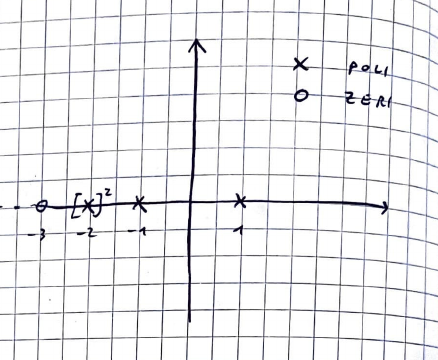
\includegraphics[width=0.75\linewidth]{automatica_mod_1_tex_assets/qa_p16_fig1.png}\par
\end{center}

\[G(0)=k_1\frac{\prod(1+\tau_{z_i}0)}{\prod(1+\tau_{p_i}0)}
=k_1\frac{\prod1}{\prod1}=k_1.\]
\emph{Nota di trascrizione (pp.~16--17): compaiono anche le scritture $Y(0)=G(0)U(0)$ e
\[G(0)=\frac{Y(0)}{U(0)}=\frac{s^{-1}y(\infty)}{s^{-1}u(\infty)}.\]
Per l'ingresso a gradino, $U(s)=M/s$ e $Y(s)$ non hanno in generale valori finiti in $s=0$; il rapporto a regime è quello ottenuto dal limite sopra.}

% Pagina originale 17
\pagina{17}
\[k_1=G(0)=\frac{y(\infty)}{u(\infty)}\qquad\text{guadagno statico}.\]
$k_1$ è il rapporto tra valore finale dell'uscita e valore finale dell'ingresso. Se $k_1>1$ l'uscita sarà amplificata ($y(\infty)>u(\infty)$); se $k_1\le1$ sarà attenuata ($y(\infty)\le u(\infty)$).
\subsection*{Velocità del sistema}
Più il polo è lontano dall'asse immaginario, più veloce sarà il sistema a portarsi a regime. Nel disegno $p_2<p_1<0$ e la risposta relativa a $p_2$ decade più rapidamente.
\subsection*{Antitrasformata di Laplace}
\[\mathcal L^{-1}\{F(s)\}=f(t)=\frac1{2\pi j}\int_{\sigma_0-j\infty}^{\sigma_0+j\infty}F(s)e^{st}ds.\]
$Y(s)=\frac ba U(s)+\frac ca$. Essendo $U(s)$ una funzione razionale fratta, $Y(s)$ sarà lo stesso:
\[\mathcal L^{-1}\{Y(s)\}=\mathcal L^{-1}\left\{\frac{N(s)}{D(s)}\right\},\qquad N,D\text{ polinomi in }s.\]
$Y(s)$ può essere propria o strettamente propria. Se propria:
\[Y(s)=q_0+\frac{R(s)}{D(s)}\Rightarrow y(t)=q_0\delta(t)+\mathcal L^{-1}\left\{\frac{R(s)}{D(s)}\right\},\quad\deg R<\deg D.\]

\begin{center}
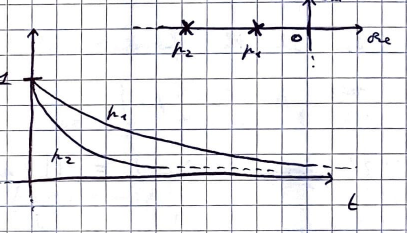
\includegraphics[width=0.75\linewidth]{automatica_mod_1_tex_assets/qa_p17_fig1.png}\par
\end{center}

% Pagina originale 18
\pagina{18}
Per $Y(s)$ strettamente propria rendo $D(s)$ monico raccogliendo il coefficiente del termine di grado massimo: $D(s)=s^\ell+d_{\ell-1}s^{\ell-1}+\cdots+d_0$.
Primo caso: radici tutte distinte:
\[D(s)=\prod_i(s-p_i),\quad F(s)=\frac{N(s)}{D(s)}=\sum_{i=1}^{\ell}\frac{k_i}{s-p_i},\quad k_i\in\mathbb C.\]
\[\mathcal L^{-1}\{F(s)\}=\left[\sum_{i=1}^{\ell}k_i e^{p_it}\right]1(t).\]
Per il teorema fondamentale dell'algebra se $p_i\in\mathbb C$ anche il suo coniugato è tra le radici.
Secondo caso: radici multiple, $D(s)=\prod_i(s-p_i)^{\nu_i}$ con $\sum_i\nu_i=\ell$. Per ciascun termine:
\[\mathcal L^{-1}\left\{\frac{k}{(s-p_i)^\nu}\right\}=k\frac{t^{\nu-1}}{(\nu-1)!}e^{p_it}1(t).\]
\subsection*{Calcolo di $k_i$}
\[F(s)=\frac{N(s)}{\prod(s-p_i)}=\frac{k_1}{s-p_1}+\frac{k_2}{s-p_2}+\cdots+\frac{k_\ell}{s-p_\ell}.\]
Moltiplicando per $s-p_1$ e valutando in $s=p_1$ gli altri termini si annullano:
\[k_i=\left[(s-p_i)F(s)\right]_{s=p_i}.\]
\begin{align*}
(s-p_1)F(s)&=(s-p_1)\frac{k_1}{s-p_1}
 +(s-p_1)\frac{k_2}{s-p_2}+\cdots,\\
\left[(s-p_1)F(s)\right]_{s=p_1}
&=k_1+\left[(s-p_1)\frac{k_2}{s-p_2}\right]_{s=p_1}+\cdots=k_1.
\end{align*}
\emph{Nota di trascrizione (p.~18): lo sviluppo manoscritto del caso multiplo mostra un solo termine per polo; lo sviluppo completo, con tutte le potenze, è esplicitato alla p.~19. La proprietà dei coniugati presuppone coefficienti reali.}

\[F(s)=\frac{N(s)}{\prod_i(s-p_i)^{\nu_i}}
=\sum_{i=1}^j\frac{k_i}{(s-p_i)^{\nu_i}},\qquad
\mathcal L^{-1}\{F(s)\}=\left[\sum_{i=1}^j k_i\frac{t^{\nu_i-1}}{(\nu_i-1)!}e^{p_it}\right]1(t).\]
\emph{La riga precedente riproduce la forma abbreviata del manoscritto (p.~18); in generale, per ciascun polo multiplo occorrono anche tutte le potenze inferiori, come nella p.~19.}
% Pagina originale 19
\pagina{19}
\subsection*{Caso di poli complessi coniugati}
\[F(s)=\frac{N(s)}{\widetilde D(s)[(s-\sigma)^2+\omega^2]}=\frac{k_1}{s-\sigma-j\omega}+\frac{k_2}{s-\sigma+j\omega}+\sum_i\frac{k_i}{s-p_i}.\]
$k_1=\overline{k_2}$ perché $p_1=\overline{p_2}$. Scrivendo $k_1=u+jv$:
\begin{align*}
\mathcal L^{-1}\left\{\frac{k_1}{s-\sigma-j\omega}+\frac{k_2}{s-\sigma+j\omega}\right\}
&=[(u+jv)e^{(\sigma+j\omega)t}+(u-jv)e^{(\sigma-j\omega)t}]1(t)\\
&=e^{\sigma t}[u(e^{j\omega t}+e^{-j\omega t})+jv(e^{j\omega t}-e^{-j\omega t})]1(t)\\
&=2e^{\sigma t}(u\cos\omega t-v\sin\omega t)1(t).
\end{align*}
Dimostro che $A\cos\omega t+B\sin\omega t=R\cos(\omega t-\varphi)$. Poiché $\cos(\omega t-\varphi)=\cos\omega t\cos\varphi+\sin\omega t\sin\varphi$, segue $A=R\cos\varphi$, $B=R\sin\varphi$, $R=\sqrt{A^2+B^2}$ e $\tan\varphi=B/A$.
\[A\cos\omega t+B\sin\omega t=\sqrt{A^2+B^2}\cos(\omega t-\arctan(B/A)).\]
Pertanto il contributo coniugato è $2e^{\sigma t}|k|\cos(\omega t+\varphi_k)1(t)$.
\subsection*{Poli con molteplicità maggiore di uno}
\[F(s)=\frac{k_{i1}}{(s-p_i)^{\nu_i}}+\frac{k_{i2}}{(s-p_i)^{\nu_i-1}}+\cdots+\frac{k_{i\nu_i}}{s-p_i}+\cdots.\]
\[[(s-p_i)^{\nu_i}F(s)]_{s=p_i}=k_{i1},\qquad \frac d{ds}[(s-p_i)^{\nu_i}F(s)]=k_{i2}+2(s-p_i)k_{i3}+\cdots.\]
\paragraph{Passaggi intermedi.}
\[u e^{\sigma t}(e^{j\omega t}+e^{-j\omega t})
+jv e^{\sigma t}(e^{j\omega t}-e^{-j\omega t})
=2u e^{\sigma t}\cos(\omega t)-2v e^{\sigma t}\sin(\omega t).\]
\emph{Nota di trascrizione (p.~19): nella riga intermedia originale compare $2j^2v$; si usa $j^2=-1$. L'espressione della fase con $\arctan(B/A)$ riportata nel manoscritto richiede la scelta del quadrante appropriato.}
\[\begin{cases}A=R\cos\varphi,\\B=R\sin\varphi\end{cases}
\Longrightarrow\quad
\begin{cases}R=\sqrt{A^2+B^2},\\B/A=\tan\varphi\end{cases}
\Longrightarrow\quad
\begin{cases}R=\sqrt{A^2+B^2},\\\varphi=\arctan(B/A).\end{cases}\]
\[\left.\frac d{ds}\{F(s)(s-p_i)^{\nu_i}\}\right|_{s=p_i}
=k_{i2}+0+\cdots+0=k_{i2}.\]
% Pagina originale 20
\pagina{20}
Valutando la derivata in $s=p_i$ si ottiene $k_{i2}$. In generale:
\[k_{ij}=\frac1{(j-1)!}\left[\frac{d^{j-1}}{ds^{j-1}}\{F(s)(s-p_i)^{\nu_i}\}\right]_{s=p_i}.\]
\subsection*{Calcolare la risposta forzata a $\delta(t)$ conoscendo $G(s)$}
$y(t)=\frac d{dt}y_1(t)$, dove $y(t)$ è risposta all'impulso $\delta(t)$ e $y_1(t)$ risposta al gradino $1(t)$. Per linearità la risposta all'impulso è la derivata della risposta al gradino.
\[Y(s)=G(s)U(s)=G(s)\mathcal L\{\delta(t)\}=G(s).\]
\subsection*{Teorema dei residui}
\[\sum_{i=1}^{\ell}k_i=\begin{cases}0&n-m>1,\\b_m/a_n&n-m=1.\end{cases}\qquad y(0)=\sum_{i=1}^{\ell}k_i.\]
Per poli multipli si intende $k_i\triangleq k_{i\nu_i}$. Esempio:
\[\frac{k_1}{s-p_1}+\frac{k_2}{s-p_2}+\frac{k_{31}}{(s-p_3)^3}+\frac{k_{32}}{(s-p_3)^2}+\frac{k_{33}}{s-p_3},\qquad k_1+k_2+k_{33}=0.\]

\begin{center}
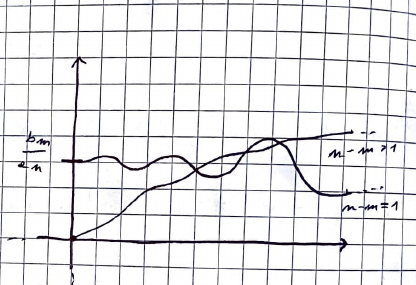
\includegraphics[width=0.75\linewidth]{automatica_mod_1_tex_assets/qa_p20_fig1.png}\par
\end{center}

% Pagina originale 21
\pagina{21}
\subsection*{Schema a blocchi}
Nodo sommatore: $E(s)=R(s)-Y(s)H(s)$.
Blocchi in serie: $G(s)=G_1(s)G_2(s)$.
Blocchi in parallelo: $U=U_1=U_2$, $Y=Y_1+Y_2=U_1G_1+U_2G_2=U(G_1+G_2)$; $G_{\rm eq}(s)=\sum_i G_i(s)$.
Retroazione:
\begin{align*}
Y(s)&=E(s)G(s)=[R(s)-X(s)]G(s)=[R(s)-Y(s)H(s)]G(s),\\
Y(s)+Y(s)H(s)G(s)&=R(s)G(s),\\
Y(s)[1+H(s)G(s)]&=R(s)G(s),\\
Y(s)&=R(s)\frac{G(s)}{1+H(s)G(s)}=R(s)G_{\rm eq}(s),\\
G_{\rm eq}(s)&=\frac{G(s)}{1\pm H(s)G(s)}.
\end{align*}
Il segno $+$ corrisponde alla retroazione negativa, il segno $-$ a quella positiva. $G$ è la FDT nel ramo diretto, $H$ nel ramo di retroazione.

\begin{center}
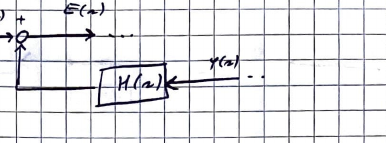
\includegraphics[width=0.75\linewidth]{automatica_mod_1_tex_assets/qa_p21_fig1.png}\par
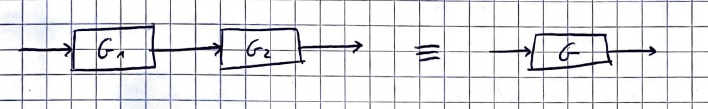
\includegraphics[width=0.75\linewidth]{automatica_mod_1_tex_assets/qa_p21_fig2.png}\par
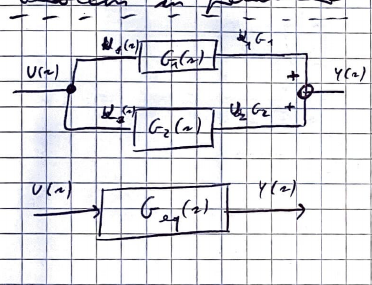
\includegraphics[width=0.75\linewidth]{automatica_mod_1_tex_assets/qa_p21_fig3.png}\par
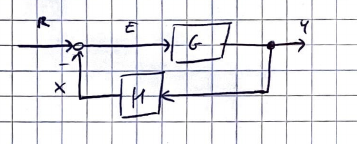
\includegraphics[width=0.75\linewidth]{automatica_mod_1_tex_assets/qa_p21_fig4.png}\par
\end{center}

% Pagina originale 22
\pagina{22}
\subsection*{Spostamento di punti di prelievo}
Un prelievo dopo $G$ si sposta prima di $G$ inserendo $G$ sul ramo prelevato. Un prelievo prima di $G$ si sposta dopo $G$ inserendo $1/G$ sul ramo prelevato.
\subsection*{Spostamento di nodi sommatori}
\[G(U+W)=GU+GW,\qquad GU+W=G(U+W/G).\]
Il nodo prima di $G$ si sposta dopo $G$ inserendo $G$ sul ramo secondario; quello dopo $G$ si sposta prima inserendo $1/G$.
\subsection*{Scambio di nodi sommatori}
Due sommatori consecutivi con ingressi $A$ e $B$ si possono scambiare. Se sono separati da $G$, spostando il secondo prima del blocco occorre inserire $1/G$ sul ramo $B$:
\[G(U+A)+B=G(U+A+B/G).\]

\begin{center}
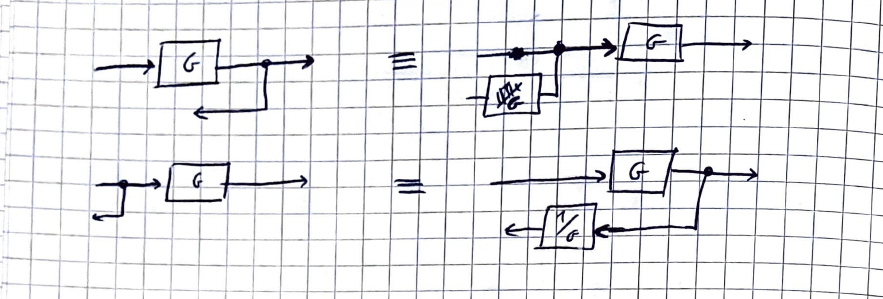
\includegraphics[width=0.86\linewidth]{automatica_mod_1_tex_assets/qa_p22_fig1.png}\par
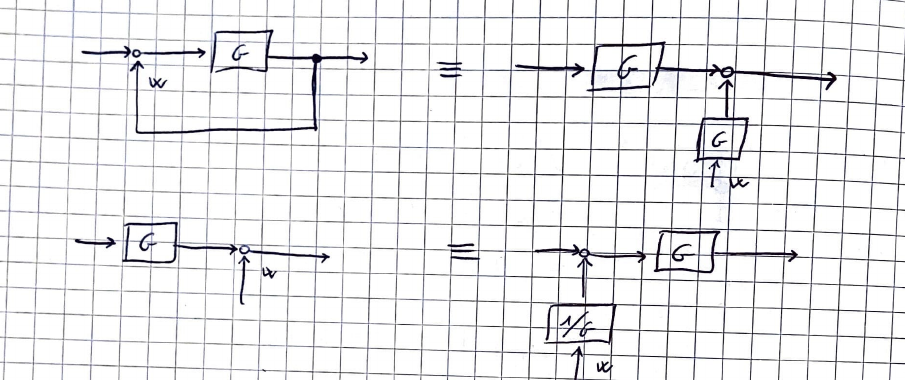
\includegraphics[width=0.86\linewidth]{automatica_mod_1_tex_assets/qa_p22_fig2.png}\par
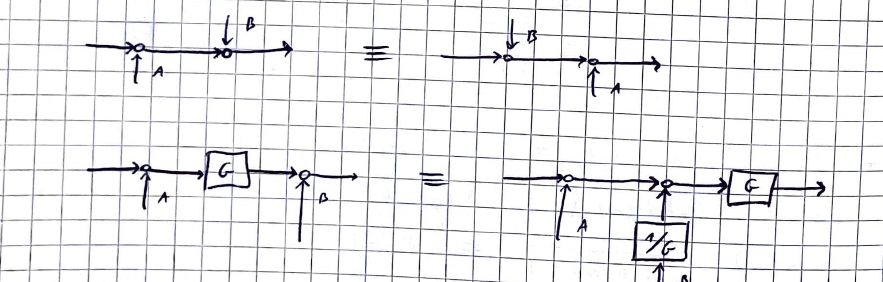
\includegraphics[width=0.86\linewidth]{automatica_mod_1_tex_assets/qa_p22_fig3.png}\par
\end{center}

% Pagina originale 23
\pagina{23}
\subsection*{Sistemi del primo ordine, $n=1$}
\[a_1y'+a_0y=b_1u'+b_0u,\quad a_1\ne0.\]
Risposta forzata (C.I. nulle):
\begin{align*}
a_1sY(s)+a_0Y(s)&=b_1sU(s)+b_0U(s),\\
Y(s)[a_1s+a_0]&=U(s)[b_1s+b_0],\\
\frac{Y(s)}{U(s)}&=\frac{b_1s+b_0}{a_1s+a_0}=\frac{b_1}{a_1}\frac{s+b_0/b_1}{s+a_0/a_1}.
\end{align*}
\[p=-\frac{a_0}{a_1},\quad z=-\frac{b_0}{b_1},\quad b_1=0\Longleftrightarrow\text{non ci sono zeri},\quad k_0=\frac{b_1}{a_1},\quad G(s)=k_0\frac{s-z}{s-p}.\]
\[G(s)=\frac{b_0}{a_0}\frac{1+(b_1/b_0)s}{1+(a_1/a_0)s},\quad G(0)=\frac{b_0}{a_0}=k_1\quad\text{(guadagno statico)}.\]
\[\tau=\frac{a_1}{a_0},\quad \alpha\tau=\frac{b_1}{b_0},\quad \alpha=\frac{b_1a_0}{b_0a_1}=\left(-\frac1z\right)(-p)=\frac pz,\quad G(s)=k_1\frac{1+\alpha\tau s}{1+\tau s}.\]
Se $b_1=0$, sistema del primo ordine privo di zeri:
\[G(s)=\frac{k_1}{1+\tau s},\quad\alpha=0.\]
\subsection*{Analisi del sistema del primo ordine privo di zeri}
\[Y_f(s)=\frac{G(s)}s=\frac{k}{s(1+\tau s)}=\frac{k_1}s+\frac{k_2}{1+\tau s}.\]
\[y_f(t)=\left(k_1+\frac{k_2}\tau e^{-t/\tau}\right)1(t)=\left(k-ke^{-t/\tau}\right)1(t).\]
$k_1=k$ e $k_2/\tau=-k$ per il teorema dei residui.
% Pagina originale 24
\pagina{24}
\[y_f(t)=k(1-e^{-t/\tau})1(t).\]
\begin{enumerate}
\item $\tau>0\Rightarrow p<0$: $y_f(\infty)=k$.
\item $\tau<0\Rightarrow p>0$: diverge, $y_f(\infty)=-\infty$ se $k>0$, $+\infty$ se $k<0$ (segni riportati come nell'originale).
\item $\tau\to\infty\Rightarrow p\to0$.
\end{enumerate}
\[a_1y'+a_0y=b_0u,\quad p=-a_0/a_1,\quad p\to0\Rightarrow a_0\to0,\quad a_1y'=b_0u.\]
\[G(s)=\frac{b_0}{a_1s}=\frac{b_0}{a_1}\frac1s=\frac ks,\quad Y(s)=\frac{k}{s^2},\quad y_f(t)=kt1(t).\]
\subsection*{Analisi della risposta ($\tau>0$)}
\[y(0)=0,\quad y(\infty)=k=G(0),\quad y(\tau)=0.63k,\quad y(2\tau)=0.86k,\quad y(3\tau)=0.95k,\quad y(5\tau)\simeq k.\]
Non esiste $\bar t$ tale che $y(\bar t)>y(\infty)=k$. Funzione monotona crescente con asintoto $y=k$.
\[\frac{dy(t)}{dt}=g(t),\qquad g(t)=\frac k\tau e^{-t/\tau}1(t).\]
$k/\tau$ è la risposta all'impulso $\delta(t)$ in $t=0$.
\autfig{24}{1}
% Pagina originale 25
\pagina{25}
\subsection*{Tempo di assestamento $t_{s,\varepsilon\%}$ (settling time)}
Esiste $t_{s,\varepsilon\%}$ tale che per ogni $t>t_{s,\varepsilon\%}$:
\[|y(t)-y(\infty)|\le\frac{\varepsilon}{100}y(\infty),\quad (1-\varepsilon/100)y(\infty)\le y(t)\le(1+\varepsilon/100)y(\infty).\]
\begin{align*}
\frac{y(t)}{y(\infty)}&\ge1-\frac\varepsilon{100},&y(t)&\ge k\left(1-\frac\varepsilon{100}\right),\\
k(1-e^{-t/\tau})1(t)&\ge k(1-\varepsilon/100)1(t),&e^{-t/\tau}&\le\frac\varepsilon{100},\\
\frac t\tau&\ge-\log\frac\varepsilon{100},&t&\ge-\tau\log\frac\varepsilon{100}.
\end{align*}
\[t_{s,\varepsilon\%}=\tau\left(-\log\frac\varepsilon{100}\right)\quad\text{(sistema primo ordine senza zeri)}.\]
\subsection*{Tempo di salita $t_r$ (rise time)}
\[t_r=t_2-t_1=t_{s,10\%}-t_{s,90\%}\simeq2.2\tau.\]
Tempo per passare dal 10\% al 90\%.
\subsection*{Tempo di ritardo $t_d$ (delay time)}
\[t_d=t_{s,50\%}=-\tau\log0.5\simeq0.7\tau.\]
\autfig{25}{1}\autfig{25}{2}
\subsection*{Risposta alla rampa $u(t)=t1(t)$}
\[Y(s)=G(s)U(s)=\frac{k}{1+\tau s}\frac1{s^2}=\frac k\tau\frac1{s^2(s+1/\tau)}=\frac{k_{11}}{s^2}+\frac{k_{12}}s+\frac{k_{21}}{s+1/\tau}.\]
\[y_f(t)=kt1(t)-k\tau1(t)+k\tau e^{-t/\tau}1(t)=k[t-\tau(1-e^{-t/\tau})]1(t).\]
% Pagina originale 26
\pagina{26}
\subsection*{Sistemi del primo ordine con uno zero}
\[G(s)=k\frac{1+\alpha\tau s}{1+\tau s},\quad z=-\frac1{\alpha\tau},\quad p=-\frac1\tau.\]
\autfig{26}{1}
\[Y(s)=G(s)U(s)=\frac{G(s)}s=k\alpha\frac{s+1/(\alpha\tau)}{s+1/\tau}\frac1s=\frac{k_1}s+\frac{k_2}{s+1/\tau}.\]
\[k_1=G(0)=k,\quad k_1+k_2=\frac{b_n}{a_n}=k\alpha,\quad k_2=k\alpha-k=k(\alpha-1).\]
\[y(t)=k[1+(\alpha-1)e^{-t/\tau}]1(t)=k[1-(1-\alpha)e^{-t/\tau}]1(t).\]
\[y(\infty)=k\quad\forall\alpha,\ \tau>0,\qquad y(0_+)=k\alpha.\]
Determino la risposta all'impulso $g(t)$:
\[g(t)=\frac d{dt}y(t)=\frac k\tau(1-\alpha)e^{-t/\tau}1(t)+k\alpha\delta(t),\quad g(0_+)=\frac k\tau(1-\alpha).\]
\[T(t)=k\alpha+\frac k\tau(1-\alpha)t,\quad T(\tau)=k\alpha+\frac k\tau(1-\alpha)\tau=k(\alpha+1-\alpha)=k.\]
Sono speculari: $\alpha_1+\alpha_2=2$.
\autfig{26}{2}
% Pagina originale 27
\pagina{27}
\[t_{s,\varepsilon\%}=-\tau\log\frac\varepsilon{100}+\tau\log|1-\alpha|.\]
Se $\log|1-\alpha|>0$ lo zero rallenta il sistema:
\[\log|1-\alpha|>0\Rightarrow\begin{cases}1-\alpha>1,\\1-\alpha<-1\end{cases}\Rightarrow\begin{cases}\alpha<0,\\\alpha>2.\end{cases}\]
Per $\alpha\in(0,2)$ lo zero velocizza l'assestamento.
\subsection*{Sistemi del secondo ordine senza zeri}
\[\frac{d^2y}{dt^2}+2\delta\omega_n\frac{dy}{dt}+\omega_n^2y=\omega_n^2u,\qquad G(s)=k\frac{\omega_n^2}{s^2+2\delta\omega_ns+\omega_n^2},\quad G(0)=k.\]
Al variare di $\delta$ e $\omega_n$ cambia la posizione dei due poli. $\delta$ è il fattore di smorzamento, adimensionale; $\omega_n$ è la pulsazione naturale [rad/s].
\[s^2+2\delta\omega_ns+\omega_n^2=0\Rightarrow p_{1,2}=-\delta\omega_n\pm\omega_n\sqrt{\delta^2-1}.\]
In base al segno di $\delta^2-1$ abbiamo:
% Pagina originale 28
\pagina{28}
\begin{enumerate}
\item Sovrasmorzato: $\delta^2>1\Rightarrow|\delta|>1$.
\item Smorzamento critico: $\delta^2=1\Rightarrow|\delta|=1$.
\item Sottosmorzato: $\delta^2<1\Rightarrow|\delta|<1$.
\end{enumerate}
\[\omega_d=\omega_n\sqrt{1-\delta^2}\le\omega_n\quad\text{pulsazione smorzata, presente nei sistemi sottosmorzati}.\]
\autfig{28}{1}
Il sistema del secondo ordine si ottiene come: serie di due sistemi del primo ordine privi di zeri con $\tau$ diversi (sovrasmorzato); serie di due sistemi del primo ordine privi di zeri con $\tau$ uguali (smorzamento critico); retroazione con ramo diretto pari a una serie di due sistemi del primo ordine privi di zeri (sottosmorzato).
\[U(s)\longrightarrow\boxed{\frac1{1+\tau_1s}}\longrightarrow\boxed{\frac1{1+\tau_2s}}\longrightarrow Y(s).\]
\begin{align*}
G(s)&=\frac1{(1+\tau_1s)(1+\tau_2s)}=\frac1{\tau_1\tau_2s^2+(\tau_1+\tau_2)s+1}\\
&=\frac1{\tau_1\tau_2}\frac1{s^2+\frac{\tau_1+\tau_2}{\tau_1\tau_2}s+\frac1{\tau_1\tau_2}}=\frac{\omega_n^2}{s^2+2\delta\omega_ns+\omega_n^2}.
\end{align*}
% Pagina originale 29
\pagina{29}
\[\begin{cases}\omega_n=\sqrt{\frac1{\tau_1\tau_2}},\\2\delta\omega_n=\frac{\tau_1+\tau_2}{\tau_1\tau_2}\end{cases}\Rightarrow\delta=\frac{\tau_1+\tau_2}{2\sqrt{\tau_1\tau_2}}.\]
\subsection*{Risposta al gradino di un sistema del secondo ordine privo di zeri: sovrasmorzato}
\[G(s)=\frac1{(1+\tau_1s)(1+\tau_2s)}=\frac1{\tau_1\tau_2}\frac1{(s+1/\tau_1)(s+1/\tau_2)},\quad\tau_1>\tau_2>0.\]
\[Y(s)=\frac{k_1}s+\frac{k_2}{s+1/\tau_1}+\frac{k_3}{s+1/\tau_2}.\]
\[k_1=G(0)=1,\quad k_2=-\frac{\tau_1}{\tau_1-\tau_2}=\frac{\tau_1}{\tau_2-\tau_1}<0,\quad k_3=\frac{\tau_2}{\tau_1-\tau_2}>0.\]
\[y(t)=\left[1-\frac{\tau_1}{\tau_1-\tau_2}e^{-t/\tau_1}+\frac{\tau_2}{\tau_1-\tau_2}e^{-t/\tau_2}\right]1(t),\quad y(0_+)=0.\]
\[g(t)=\frac d{dt}y(t)=\frac1{\tau_1-\tau_2}e^{-t/\tau_1}-\frac1{\tau_1-\tau_2}e^{-t/\tau_2}=\frac{e^{-t/\tau_1}-e^{-t/\tau_2}}{\tau_1-\tau_2}.\]
Somma algebrica delle tre funzioni:
\[y_1(t)=1(t),\quad y_2(t)=-\frac{\tau_1}{\tau_1-\tau_2}e^{-t/\tau_1}1(t),\quad y_3(t)=\frac{\tau_2}{\tau_1-\tau_2}e^{-t/\tau_2}1(t).\]
Forma a sigmoide.
\autfig{29}{1}\autfig{29}{2}
% Pagina originale 30
\pagina{30}
\subsection*{Smorzamento critico}
\[G(s)=\frac{\omega_n^2}{(s+\omega_n)^2},\quad Y(s)=\frac{\omega_n^2}{s(s+\omega_n)^2}=\frac{k_1}s+\frac{k_{21}}{(s+\omega_n)^2}+\frac{k_{22}}{s+\omega_n}.\]
\[k_1=G(0)=1,\quad k_{22}=-1\text{ per il teorema dei residui},\quad k_{21}=-\omega_n.\]
\[y(t)=[1-e^{-\omega_nt}(\omega_nt+1)]1(t),\quad y(0_+)=0,\quad y'(0_+)=0,\quad\omega_n>0.\]
\autfig{30}{1}
\subsection*{Sottosmorzati}
\[p_{1,2}=-\delta\omega_n\pm j\omega_d,\quad |p_1|=|p_2|=\sqrt{\delta^2\omega_n^2+\omega_d^2}=|\omega_n|=\omega_n.\]
\[\theta=\arctan\frac{\omega_n\sqrt{1-\delta^2}}{\delta\omega_n}=\arctan\frac{\sqrt{1-\delta^2}}\delta=\arccos\delta=\arcsin\sqrt{1-\delta^2}.\]
\[Y(s)=G(s)U(s)=\frac{G(s)}s=\frac{\omega_n^2}{(s+\delta\omega_n)^2+\omega_d^2}\frac1s=\frac{k_1}s+\frac{\alpha s+\beta}{(s+\delta\omega_n)^2+\omega_d^2}.\]
\[k_1=G(0)=1,\qquad \left.(\alpha s+\beta)\right|_{s=-\delta\omega_n+j\omega_d}=\left.\frac{\omega_n^2}s\right|_{s=-\delta\omega_n+j\omega_d}.\]
% Pagina originale 31
\pagina{31}
\[\begin{cases}-\alpha\delta\omega_n+\beta=-\delta\omega_n,\\j\omega_d\alpha=-j\omega_d\end{cases}\Rightarrow\begin{cases}\alpha=-1,\\\beta=-2\delta\omega_n.\end{cases}\]
\[y(t)=\left[1-\frac{e^{-\delta\omega_nt}}{\sqrt{1-\delta^2}}\sin(\omega_dt+\theta)\right]1(t).\]
Se $\delta=0$:
\[y(t)=[1-\sin(\omega_nt+\pi/2)]1(t)=[1-\cos(\omega_nt)]1(t).\]
\[\lim_{t\to\infty}y(t)=1,\quad y(0_+)=1-\frac{\sin\theta}{\sqrt{1-\delta^2}}=0.\]
\paragraph{Nota di lettura, pagina 31} In due denominatori della scansione il segno sotto radice sembra $+$; si è riportato $\sqrt{1-\delta^2}$ coerentemente con le altre righe della stessa derivazione.
Massimi e minimi si trovano a $k\pi/\omega_d$.
\autfig{31}{1}
\subsection*{Inviluppi}
\[\left|\frac{e^{-\delta\omega_nt}}{\sqrt{1-\delta^2}}\sin(\omega_dt+\theta)\right|=|y(t)-1|=|1-y(t)|.\]
\[\left|\frac{e^{-\delta\omega_nt}}{\sqrt{1-\delta^2}}\right||\sin(\omega_dt+\theta)|\le\frac{e^{-\delta\omega_nt}}{\sqrt{1-\delta^2}}.\]
\[y(t)\in\left[1-\frac{e^{-\delta\omega_nt}}{\sqrt{1-\delta^2}},\ 1+\frac{e^{-\delta\omega_nt}}{\sqrt{1-\delta^2}}\right].\]
Tocca gli inviluppi quando $|\sin(\omega_dt+\theta)|=1$:
\[\omega_dt+\theta=(k+1/2)\pi\Rightarrow \bar t=\frac{\pi(k+1/2)-\theta}{\omega_d},\quad k\in\mathbb N.\]
% Pagina originale 32
\pagina{32}
\subsection*{Massimi e minimi locali}
\begin{align*}
\frac{dy(t)}{dt}=0&\Rightarrow\frac d{dt}\left[\frac{e^{-\delta\omega_nt}}{\sqrt{1-\delta^2}}\sin(\omega_dt+\theta)\right]=0\\
&\Rightarrow\frac{\omega_ne^{-\delta\omega_nt}}{\sqrt{1-\delta^2}}[\delta\sin(\omega_dt+\theta)-\sqrt{1-\delta^2}\cos(\omega_dt+\theta)]=0\\
&\Rightarrow\frac{\omega_ne^{-\delta\omega_nt}}{\sqrt{1-\delta^2}}\sin(\omega_dt+\theta-\theta)=0\\
&\Rightarrow\sin(\omega_dt)=0\Rightarrow\omega_dt=k\pi\Rightarrow\bar t=\frac{k\pi}{\omega_d}.
\end{align*}
\subsection*{Tempo di picco (peak time)}
\[t_p=t_{\max}-t_0=\left.\frac{k\pi}{\omega_d}\right|_{k=1}-\left.\frac{k\pi}{\omega_d}\right|_{k=0}=\frac\pi{\omega_d}.\]
\[t_1<t_3\Longleftrightarrow e^{-\delta\omega_nt_1}>e^{-\delta\omega_nt_3}\Rightarrow\max_{k=1}>\max_{k=3}.\]
Tutti i sistemi del secondo ordine hanno $y(0_+)=y'(0_+)=0$.
\autfig{32}{1}
\subsection*{Tempo di salita (rise time)}
Differentemente dal tempo di salita nei sistemi del primo ordine, $t_r$ è il tempo minimo che ci mette il sistema a raggiungere $y(\infty)$.
\[y(t_r)=y(\infty)=1,\quad 1-\frac{e^{-\delta\omega_nt_r}}{\sqrt{1-\delta^2}}\sin(\omega_dt_r+\theta)=1.\]
\[\omega_dt_r+\theta=k\pi\Rightarrow t_r=\frac{k\pi-\theta}{\omega_d},\quad|t_r-t_p|=\frac\theta{\omega_d},\quad t_r<t_p.\]
% Pagina originale 33
\pagina{33}
\subsection*{Tempo di assestamento $t_{s,\varepsilon\%}$}
Considero gli inviluppi, $y(\infty)=1$:
\begin{align*}
1+\frac{e^{-\delta\omega_nt}}{\sqrt{1-\delta^2}}&=y(\infty)\left(1+\frac\varepsilon{100}\right),\\
\frac{e^{-\delta\omega_nt}}{\sqrt{1-\delta^2}}&=\frac\varepsilon{100},\\
-\delta\omega_nt&=\log\frac{\varepsilon\sqrt{1-\delta^2}}{100},\\
t_{s,\varepsilon\%}&=-\frac{\log[\varepsilon\sqrt{1-\delta^2}/100]}{\delta\omega_n}=-\tau\log\frac{\varepsilon\sqrt{1-\delta^2}}{100},\quad\tau=\frac1{\delta\omega_n}.
\end{align*}
\[\delta\ll1\Rightarrow t_{s,\varepsilon\%}\simeq-\tau\log\frac\varepsilon{100}=-\frac1{\delta\omega_n}\log\frac\varepsilon{100}.\]
Ricorda che $-\delta\omega_n=\operatorname{Re}(p_1)$, $\omega_d=\operatorname{Im}(p_1)$. In base alla posizione dei poli posso calcolare i tempi di salita, di picco, minimi e massimi, ecc.
\subsection*{Luoghi a $\delta$ e $\omega_n$ costante}
\[\delta_1=\cos\theta_1=0,\quad\theta_1=\pi/2;\qquad \delta_3=1=\cos\theta_3,\quad\theta_3=0;\qquad\delta_2=\sqrt2/2=\cos\theta_2,\quad\theta_2=\pi/4.\]
\autfig{33}{1}
% Pagina originale 34
\pagina{34}
\subsection*{Massima sovraelongazione percentuale $M_{p\%}$}
\[M_{p\%}=\frac{y(t_p)-y(\infty)}{y(\infty)}100.\]
$y(\infty)$ è il valore a valle, $y(t_p)$ il massimo assoluto.
\begin{align*}
y(t_p)=y(\pi/\omega_d)&=1-\frac{e^{-\delta\omega_n\pi/\omega_d}}{\sqrt{1-\delta^2}}\sin(\pi+\theta)\\
&=1+e^{-\delta\omega_n\pi/\omega_d}\frac{\sin\theta}{\sqrt{1-\delta^2}}=1+e^{-\cot\theta\,\pi},\\
M_{p\%}&=\frac{1+e^{-\cot\theta\,\pi}-1}1\,100=100e^{-\cot\theta\,\pi}.
\end{align*}
$M_{p\%}=100\%$ per $\delta=0$; $M_{p\%}\to0$ per $\delta\to1$.
\autfig{34}{1}
\subsection*{Sistemi del secondo ordine con uno zero}
\[G(s)=\frac{\omega_n^2(1+\tau s)}{s^2+2\delta\omega_ns+\omega_n^2},\quad G(0)=1=k,\quad z=-1/\tau.\]
\[G(s)=\frac{\omega_n^2}{s^2+2\delta\omega_ns+\omega_n^2}+\frac{\tau s\omega_n^2}{s^2+2\delta\omega_ns+\omega_n^2}=\bar G(s)+\tau s\bar G(s).\]
\[\mathcal L^{-1}\{\tau s\bar Y(s)\}=\tau\frac{d\bar y}{dt}=\tau\bar y'(t),\quad y(t)=\bar y(t)+\tau\bar y'(t).\]
Più grande è $\tau$ più sarà influenzato dallo zero il sistema (più grande è $\tau$, più vicino a zero è $z$).
\autfig{34}{2}
% Pagina originale 35
\pagina{35}
$\tau>0\Rightarrow z<0$. Nota: parte con pendenza positiva; $M_{p\%,1}>M_{p\%,0}$; $t_{p,1}<t_{p,0}$; $y_1(t)=y_0(t)$ quando $t=k\pi/\omega_d$; $t_{s,\varepsilon\%}$ aumenta.
$\tau<0\Rightarrow z>0$: $y_1'(0_+)<0$ e c'è una sottoelongazione.
\autfig{35}{1}\autfig{35}{2}
\subsection*{Stabilità}
Un sistema è:
\begin{enumerate}
\item semplicemente stabile se $\forall u(t)\in\mathcal S_\ell\ \exists M_y>0$ tale che $|y(t)|\le M_y$ per ogni $t$;
\item asintoticamente stabile se è semplicemente stabile e $\lim_{t\to\infty}y(t)=0$;
\item instabile se esistono C.I. tali che l'uscita $y(t)$ diverge.
\end{enumerate}
$\mathcal S_\ell$ contiene tutti i segnali a supporto limitato: $u(t)=f(t)$ per $0\le t\le\tau$, zero altrove.
Trovo l'espressione in fratti semplici di $Y_\ell(s)$:
\[Y_\ell(s)=\left(\sum_{i=1}^n a_i\sum_{j=0}^{i-1}s^jD^{(i-j-1)}y(0)\right)\left(\sum_{i=0}^na_is^i\right)^{-1}=\frac{N(s)}{a(s)}.\]
\[y_\ell(t)=\sum_{i=1}^\ell\sum_{j=1}^{\nu_i}R_{ij}t^{\nu_i-j}e^{p_it},\quad R_{ij}=\frac{k_{ij}}{(\nu_i-j)!}.\]
\[y_\ell(t)=\sum_{i=1}^\ell m_i(t)e^{p_it},\qquad m_i(t)=\sum_{j=1}^{\nu_i}R_{ij}t^{\nu_i-j}.\]

% Pagina originale 36
\pagina{36}
Affinché $y_\ell$ sia asintoticamente stabile:
\[
m_i(t)e^{p_it}\to0\quad\forall i,
\qquad e^{p_it}\to0\quad\Longrightarrow\quad\operatorname{Re}(p_i)<0\quad\forall i.
\]
\subsection*{Classificazione della stabilità di un sistema LTI in base ai poli di $G(s)$}
\begin{enumerate}
\item Sistema asintoticamente stabile $\Longleftrightarrow\forall i:\operatorname{Re}(p_i)<0$.
\item Sistema instabile $\Longleftrightarrow\exists p\in\{p_i\}:\operatorname{Re}(p)>0$, oppure
$\exists i:\operatorname{Re}(p_i)=0\land r_i\geq1$.
\item Sistema semplicemente stabile $\Longleftrightarrow\forall i:\operatorname{Re}(p_i)<0$, oppure
$(\operatorname{Re}(p_i)=0\land r_i=1)$.
\end{enumerate}
% La scansione scrive r_i >= 1 nel criterio di instabilità e r_i=1 nel criterio di stabilità semplice; disuguaglianza conservata.
\paragraph{Esempi}
\begin{center}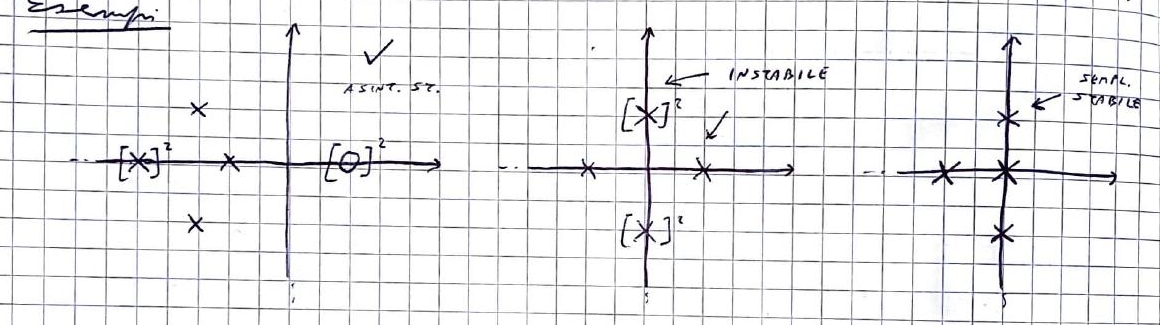
\includegraphics[width=\linewidth]{automatica_mod_1_tex_assets/b36_p36_1.png}\end{center}
\subsection*{Stabilità BIBO (Bounded Input Bounded Output)}
Per ogni $u(t)$ limitato in ampiezza esiste $y(t)$ limitata in ampiezza.
\[
\text{Un sistema è stabile BIBO}\quad\Longleftrightarrow\quad g(t)\to0.
\]
Stabilità BIBO $=$ sistema asintoticamente stabile.
\subsection*{Analisi della stabilità di un sistema ad anello chiuso}
\begin{center}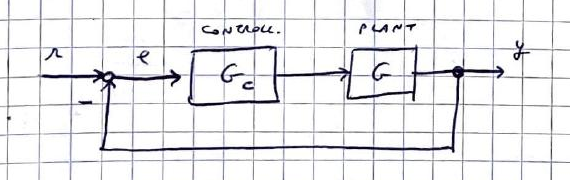
\includegraphics[width=.7\linewidth]{automatica_mod_1_tex_assets/b36_p36_2.png}\end{center}
\[
G(s)=\frac{b(s)}{a(s)}=k\frac{\prod_{i=1}^{m}(s-z_i)}{\prod_{i=1}^{n}(s-p_i)}.
\]
\begin{align*}
G_0(s)&=\frac{G_c(s)G(s)}{1+G_c(s)G(s)}\\
&=\frac{\frac{b_c(s)}{a_c(s)}\frac{b(s)}{a(s)}}
{1+\frac{b_c(s)}{a_c(s)}\frac{b(s)}{a(s)}}
=\frac{b_c(s)b(s)}{a_c(s)a(s)+b_c(s)b(s)}.
\end{align*}
$\text{Zeri di }G_0(s)$: quelli del numeratore $b_c(s)b(s)$.
% Pagina originale 37
\pagina{37}
La retroazione non sposta gli zeri, sposta i poli.
I nuovi poli sono le soluzioni dell'equazione caratteristica $a_0(s)=0$.
$a_0(s)$ è il polinomio caratteristico:
\[
a_0(s)=a(s)a_c(s)+b_c(s)b(s)=0.
\]
\subsection*{Lemma di Routh}
Condizione necessaria, non sufficiente, per la stabilità asintotica di un sistema LTI è che il polinomio caratteristico abbia tutti i coefficienti dello stesso segno e non nulli.
Negando l'affermazione precedente troviamo una condizione sufficiente affinché il sistema non sia asintoticamente stabile: basta un coefficiente nullo o discorde dagli altri.
\subsection*{Criterio di Routh--Hurwitz}
\[
a_0(s)=a_ns^n+a_{n-1}s^{n-1}+a_{n-2}s^{n-2}+a_{n-3}s^{n-3}+\cdots+a_1s+a_0.
\]
\[
\begin{array}{c|cccccc}
n&a_n&a_{n-2}&\cdots&\cdots&a_0&0\\
n-1&a_{n-1}&a_{n-3}&\cdots&\cdots&0&0\\
n-2&b_{n-2}&b_{n-4}&\cdots&\cdots&0&0\\
n-3&c_{n-3}&c_{n-5}&\cdots&\cdots&0&0\\
\vdots&\vdots&\vdots&\cdots&\cdots&\vdots&\vdots\\
1&\cdots&\cdots&0&0&0&0\\
0&\cdots&0&0&0&0&0
\end{array}
\]
\[
b_{n-2}=-\frac{\begin{vmatrix}a_n&a_{n-2}\\a_{n-1}&a_{n-3}\end{vmatrix}}{a_{n-1}},
\qquad b_{n-4}=-\frac{\begin{vmatrix}a_n&a_{n-4}\\a_{n-1}&a_{n-5}\end{vmatrix}}{a_{n-1}},
\]
\[
c_{n-3}=-\frac{\begin{vmatrix}a_{n-1}&a_{n-3}\\b_{n-2}&b_{n-4}\end{vmatrix}}{b_{n-2}},
\qquad c_{n-5}=-\frac{\begin{vmatrix}a_{n-1}&a_{n-5}\\b_{n-2}&b_{n-6}\end{vmatrix}}{b_{n-2}}.
\]
La prima colonna è chiamata sequenza di Routh:
\[
S_{\mathrm{Routh}}=(a_n,a_{n-1},b_{n-2},c_{n-3},d_{n-4},\ldots,y_{n-1},z_0).
\]
% Pagina originale 38
\pagina{38}
\subsection*{Teorema di Routh--Hurwitz}
Per ogni variazione di segno nella sequenza di Routh corrisponde una radice di $a_0(s)$ a parte reale positiva.
Per ogni permanenza di segno corrisponde una radice a parte reale negativa.
\paragraph{Esempio}
\[
S=(3,-3,4,5,-1,3).
\]
Variazioni: $3\to-3$, $-3\to4$, $5\to-1$, $-1\to3$ ($p_1,p_2,p_4,p_5>0$); permanenza: $4\to5$ ($p_3<0$).
Ci sono quattro poli positivi ed uno negativo.
Un sistema LTI è asintoticamente stabile se ogni elemento della sequenza di Routh ha sempre lo stesso segno.
Se il primo elemento di una riga è nullo posso sostituire a zero $\varepsilon>0$ e calcolare i termini della riga successiva senza dividere per $\varepsilon$ il risultato e sostituendo $\varepsilon$ con zero.
Se ho frazioni posso moltiplicare tutta la riga per un numero reale positivo.
Posso sommare una riga per se stessa traslata di $h$ posizioni e moltiplicata per $(-1)^h$.
Se ho una riga tutta nulla questa sarà per forza in posizioni dispari (se fosse in posizione pari ho $a_0=0$ e quindi posso raccogliere $s$ e fare Routh su $\widetilde a(s)=a(s)/s$).
Posso sostituire l'equazione della riga sopra con $p(s)=b(s)$, calcolarmi la derivata in $s$ e mettere i coefficienti nella riga tutta nulla.
% La notazione manoscritta accanto a b(s) nella regola della riga nulla è poco chiara; la procedura e il simbolo b(s) sono riportati fedelmente.
% Pagina originale 39
\pagina{39}
\subsection*{Stabilità di un sistema con parametri}
Affronto questa parte con esempi pratici.
\[
G(s)=\frac1{s(s+1)(s+2)}.
\]
\begin{center}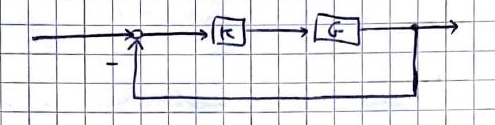
\includegraphics[width=.72\linewidth]{automatica_mod_1_tex_assets/b36_p39_1.png}\end{center}
\begin{align*}
G_0(s)&=\frac{kG}{1+kG}=\frac{k}{s(s+1)(s+2)+k}
=\frac{k}{s^3+3s^2+2s+k},\\
a_0(s)&=s^3+3s^2+2s+k.
\end{align*}
\[
\begin{array}{c|ccc}
3&1&2&0\\2&3&k&0\\1&6-k&0&0\\0&k&0&0
\end{array},\qquad
b=-\frac{\begin{vmatrix}1&2\\3&k\end{vmatrix}}3=\frac{6-k}{3},
\qquad b'=3b=6-k.
\]
\[
S=(1,3,6-k,k).
\]
È stabile se $k\in(0,6)$.
\[
\begin{array}{c|ccc}
&k<0&0<k<6&k>6\\\hline
1&+&+&+\\3&+&+&+\\6-k&+&+&-\\k&-&+&+
\end{array}
\]
$k<0$: instabile con un polo positivo; $0<k<6$: stabile; $k>6$: instabile con due poli positivi.
Trovo i valori zero e sei:
\[
k=0\quad\Longrightarrow\quad
 a_0(s)=s^3+3s^2+2s=s(s^2+3s+2)=s(s+2)(s+1).
\]
Semplicemente stabile.
\[
k=6\quad\Longrightarrow\quad a_0(s)=s^3+3s^2+2s+6.
\]
\[
\begin{array}{c|cc}3&1&2\\2&3&6\\1&3&0\\0&6&0\end{array},
\qquad b(s)=3s^2+6,
\qquad b(z)=3z+6\xrightarrow{=0}z=-2,
\qquad b'(z)=3.
\]
\[
p=\pm j\sqrt2.
\]
\begin{center}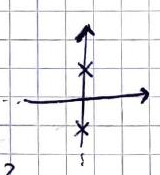
\includegraphics[width=.25\linewidth]{automatica_mod_1_tex_assets/b36_p39_2.png}\end{center}
Semplicemente stabile: tutte permanenze, ma elemento nullo in $S$, quindi non è asintoticamente stabile.
% Pagina originale 40
\pagina{40}
\subsection*{Precisione dei sistemi di controllo a regime permanente}
\begin{center}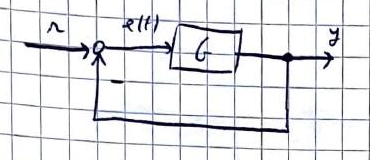
\includegraphics[width=.55\linewidth]{automatica_mod_1_tex_assets/b36_p40_1.png}\end{center}
Assumo che il sistema sia asintoticamente stabile.
Suppongo un sistema con retroazione unitaria $H(s)=1$.
Valuto l'errore a regime:
\[
e(\infty)=\lim_{s\to0}sE(s).
\]
\begin{align*}
Y(s)&=G(s)E(s)\quad\Longrightarrow\quad E(s)=\frac{Y(s)}{G(s)},\\
Y(s)&=G_0(s)R(s)=\frac{G(s)}{1+G(s)}R(s)
\quad\Longrightarrow\quad E(s)=\frac1{1+G(s)}R(s).
\end{align*}
I poli di $E(s)$ sono gli stessi di $G_0(s)$ più quelli di $R(s)$.
$E(s)$ è instabile se $G_0(s)$ è instabile.
Definisco tre errori:
\begin{itemize}
\item errore di posizione: $r(t)=1(t)$, $e_p$;
\item errore di velocità: $r(t)=t\,1(t)$, $e_v$;
\item errore di accelerazione: $r(t)=\frac{t^2}{2}\,1(t)$, $e_a$.
\end{itemize}
\subsection*{Errore di posizione $e_p$}
\[
e(\infty)=\lim_{s\to0}sE(s)
=\lim_{s\to0}s\frac1{1+G(s)}R(s)
=\frac1{1+G(s)}\mathrel{\triangleq}k_p.
\]
% La prima catena manoscritta attribuisce k_p a 1/(1+G(s)); sotto definisce k_p=G(0). Entrambe le righe sono conservate.
\[
k_p=\lim_{s\to0}G(s)=G(0)\qquad\text{costante di posizione},
\]
\[
e(\infty)=\frac1{1+k_p}\qquad\left(=\frac1{1+k_pH(s)}\right).
\]
Se $\mu=0$ ($\mu$ è il tipo del sistema: il numero di poli nell'origine di $G(s)$), $G(0)\in\mathbb R$.
Se $\mu\geq1$:
\[
G(0)=\lim_{s\to0}k\frac{\prod_i(s-z_i)}{s\prod_i(s-p_i)}=\infty.
\]
Quindi
\[
k_p\to\infty\quad\Longrightarrow\quad
 e(\infty)=\frac1{1+k_p}\to0.
\]
% Pagina originale 41
\pagina{41}
\[
e_p(\infty)=\begin{cases}\frac1{1+G(0)}&\mu=0,\\0&\mu\geq1,\end{cases}
\qquad\text{quando }r(t)=1(t).
\]
\subsection*{Errore di velocità $e_v$}
\[
E(s)=\frac1{1+G(s)}\frac1{s^2}.
\]
\begin{align*}
e(\infty)&=\lim_{s\to0}\frac1{1+G(s)}\cdot\frac1s
=\lim_{s\to0}\frac1{s+sG(s)}
=\lim_{s\to0}\frac1{sG(s)},\\
k_v&\mathrel{\triangleq}\lim_{s\to0}sG(s),\qquad
 e(\infty)=e_v=\frac1{k_v}.
\end{align*}
\begin{align*}
\mu=0&:\quad k_v=0\quad\Longrightarrow\quad e_v(\infty)\to\infty,\\
\mu=1&:\quad k_v=\lim_{s\to0}s\frac1s\overline G(s)=\overline G(0)\in\mathbb R,
\quad e(\infty)=\frac1{\overline G(0)}\in\mathbb R,\\
\mu\geq2&:\quad k_v=\lim_{s\to0}s\frac1{s^2}\overline G(s)=\infty
\quad\Longrightarrow\quad e(\infty)\to0.
\end{align*}
\[
e(\infty)=\begin{cases}\infty&\mu=0,\\\frac1{\overline G(0)}&\mu=1,\\0&\mu\geq2.\end{cases}
\]
\subsection*{Errore di accelerazione $e_a$}
\[
E(s)=\frac1{1+G(s)}\frac1{s^3}.
\]
\[
e(\infty)=\lim_{s\to0}sE(s)
=\frac1{1+G(s)}\cdot\frac1{s^2}
=\lim_{s\to0}\frac1{s^2G(s)},
\qquad k_a\mathrel{\triangleq}\lim_{s\to0}s^2G(s),\qquad e(\infty)=\frac1{k_a}.
\]
\begin{align*}
\mu=0&\Longrightarrow k_a=0\Longrightarrow e(\infty)\to\infty,\\
\mu=1&\Longrightarrow k_a=0\Longrightarrow e(\infty)\to\infty,\\
\mu=2&\Longrightarrow k_a=\overline G(0)\Longrightarrow
 e(\infty)=\frac1{\overline G(0)}\in\mathbb R,\\
\mu\geq3&\Longrightarrow k_a\to\infty\Longrightarrow e(\infty)\to0.
\end{align*}
% Pagina originale 42
\pagina{42}
\[
\begin{array}{c|cccc}\mu&0&1&2&3\\\hline
 e_p&\frac1{1+G(0)}&0&0&0\\
 e_v&\infty&\frac1{\overline G(0)}&0&0\\
 e_a&\infty&\infty&\frac1{\overline G(0)}&0
\end{array}
\]
\subsection*{Errore a regime permanente nei sistemi di controllo a retroazione non unitaria}
Tipicamente $H(s)$ è di tipo zero, quindi $H(0)$ è il guadagno statico.
\[
\widehat y(\infty)=H(0)y(\infty)\quad\Longrightarrow\quad H(0)=\gamma,
\qquad e(t)=r(t)-\gamma y(t).
\]
\[
e(t)=0\quad\Longrightarrow\quad y(t)=\frac{r(t)}\gamma.
\]
\begin{center}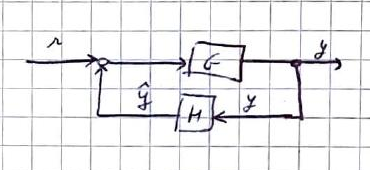
\includegraphics[width=.55\linewidth]{automatica_mod_1_tex_assets/b36_p42_1.png}\end{center}
\[
G_{\mathrm{eq}}(s)=\frac{\gamma G(s)}{1+G(s)[H(s)-\gamma]}.
\]
\paragraph{Dimostrazione}
\begin{center}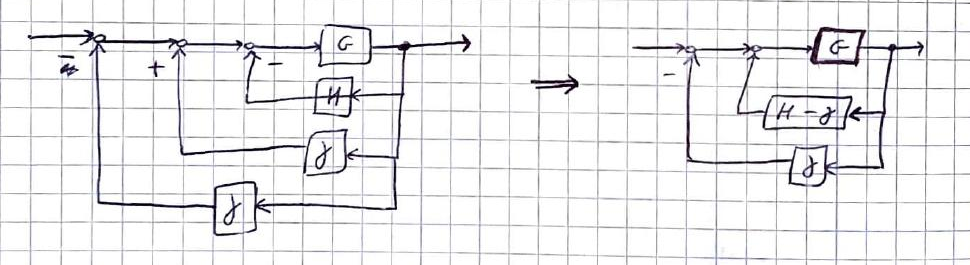
\includegraphics[width=\linewidth]{automatica_mod_1_tex_assets/b36_p42_2.png}\end{center}
\begin{center}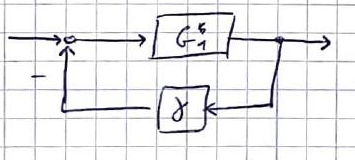
\includegraphics[width=.55\linewidth]{automatica_mod_1_tex_assets/b36_p42_3.png}\end{center}
Con
\[
G_1^\gamma=\frac G{1+G(H-\gamma)}.
\]
\begin{center}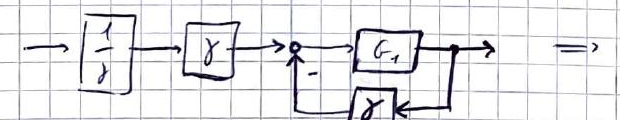
\includegraphics[width=.8\linewidth]{automatica_mod_1_tex_assets/b36_p42_4.png}\end{center}
\begin{center}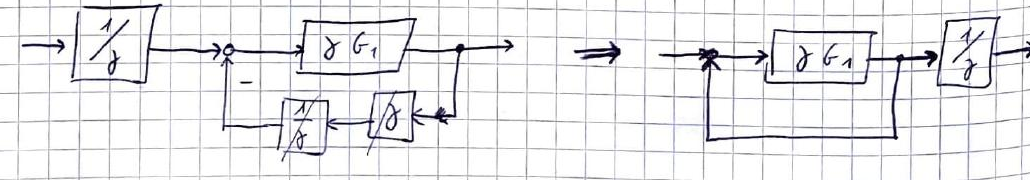
\includegraphics[width=\linewidth]{automatica_mod_1_tex_assets/b36_p42_5.png}\end{center}
% Pagina originale 43
\pagina{43}
\subsection*{Reiezione dei disturbi a regime}
Un sistema ad anello aperto non può reiettare disturbi.
\begin{center}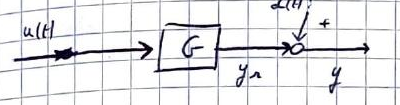
\includegraphics[width=.55\linewidth]{automatica_mod_1_tex_assets/b36_p43_1.png}\end{center}
\[
y(t)=y_r(t)+d(t),\qquad
 d(t)=1(t)\quad\Longrightarrow\quad y(\infty)=y_r(\infty)+1.
\]
Non posso reiettare nessun disturbo al di fuori dell'anello di controllo.
\begin{center}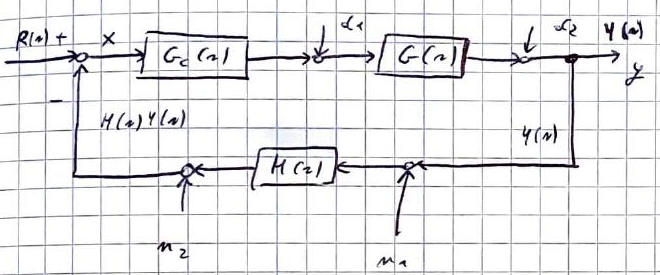
\includegraphics[width=.85\linewidth]{automatica_mod_1_tex_assets/b36_p43_2.png}\end{center}
Uso il PSE. Trovo $Y_{d_1}(s)$:
\begin{align*}
Y(s)&=[X(s)G_c(s)+D(s)]G(s),\\
Y(s)&=[(R(s)-H(s)Y(s))G_c(s)+D(s)]G(s),\\
Y(s)&=R(s)G_c(s)G(s)-H(s)Y(s)G_c(s)G(s)+D(s)G(s),\\
Y(s)(1+H(s)G_c(s)G(s))&=R(s)G_c(s)G(s)+D(s)G(s),\\
G_d(s)&=\frac{Y(s)}{D(s)}=\frac{G(s)}{1+H(s)G(s)G_c(s)}.
\end{align*}
Nel calcolo di $G_d$ pongo $R(s)=0$.
$a_0(s)$ deve avere tutti i poli nel semipiano aperto di sinistra.
Trovo
\[
Y_r(s)=\frac{G_cG}{1+HG_cG}.
\]
$Y_r(s)$ deve essere asintoticamente stabile.
Considero $D_1(s)=1/s^k$ con $k\geq1$. Vediamo per ogni $k$ quando riesco a reiettare $d_1(t)$.
% Pagina originale 44
\pagina{44}
\[
k=1,\qquad D_1(s)=\frac1s,\qquad d(t)=1(t).
\]
\[
y_{d_1}(\infty)=\lim_{s\to0}sY(s)
=\lim_{s\to0}s\frac{G(s)}{1+G(s)H(s)G_c(s)}\frac1s.
\]
Ipotizzo un polo di $G(s)$ nell'origine:
\begin{align*}
y_{d_1}(\infty)&=\lim_{s\to0}\frac{G(s)\to\infty}{1+H(s)G_c(s)G(s)}\\
&=\lim_{s\to0}\frac{G(s)}{H(s)G(s)G_c(s)}
=\lim_{s\to0}\frac1{H(s)G_c(s)}.
\end{align*}
Ipotizzo $H$ di tipo zero ($\mu_H=0$):
\[
y_{d_1}(\infty)=\frac1{H(0)}\lim_{s\to0}\frac1{G_c(s)}.
\]
Se $G_c(s)$ è di tipo zero:
\[
y_{d_1}(\infty)=\frac1{H(0)G_c(0)}\in\mathbb R.
\]
Quindi, se $G_c(s)$ è di tipo zero, $1(t)$ non è reiettabile.
Se $G_c(s)$ è di tipo uno, $y_{d_1}(\infty)=0$: se $G_c(s)$ è di tipo uno, $1(t)$ è reiettabile.
In generale: se $d_1(t)$ è di tipo $k$, è reiettabile solo se $G_c(s)$ (funzione di trasferimento a monte) è di tipo $\overline k\geq k$.
Trovo ora
\[
Y_{d_2}(s)=D_2(s)\frac1{1+HG_cG},\qquad
G_{d_2}(s)=\frac1{1+H(s)G(s)G_c(s)}.
\]
\[
y_{d_2}(\infty)=G_{d_2}(s\to0)
=\lim_{s\to0}\frac1{1+H(s)G(s)G_c(s)}.
\]
\[
y_{d_2}(\infty)\to0\quad\Longleftrightarrow\quad
G(s)G_c(s)\text{ ha almeno un polo nell'origine}.
\]
% Pagina originale 45
\pagina{45}
Generalizzando: se $d_2(t)$ è di tipo $k$, è reiettabile se è a monte di una funzione di trasferimento di tipo $\overline k\geq k$.
Solitamente il controllore ha tipo $\mu_c\geq\mu$, il tipo dell'attuatore, perché ``comanda'' quelli successivi.
\subsection*{Disturbi sul ramo di retroazione}
\begin{center}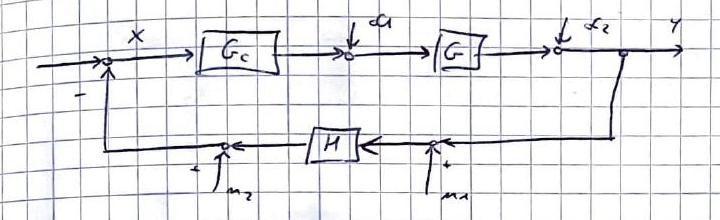
\includegraphics[width=.88\linewidth]{automatica_mod_1_tex_assets/b36_p45_1.png}\end{center}
\[
Y_{m_1}(s)=\frac{G_cGH}{1+G_cGH}.
\]
% Nella prima espressione originale manca il meno; la derivazione seguente lo include.
\begin{align*}
X(s)G_cG&=Y,\\
X(s)&=R(s)-Y(s)H(s)-N_1(s)H(s),\\
Y&=-Y(s)H(s)G_cG-N_1(s)H(s)GG_c,\\
Y(1+HG_cG)&=-N_1HG_cG,\\
Y_{m_1}&=-N_1\left(\frac{HG_cG}{1+HG_cG}\right).
\end{align*}
Se $G_c$ e $G$ devono reiettare $d_1$ e $d_2$ dovranno avere tipo $\mu\geq1$, quindi a $s\to0$:
\[
|G_cG|\gg1\qquad(G_cG\to\infty),
\]
\[
Y_{m_1}(s)\simeq-N_1
\quad\Longrightarrow\quad y_{m_1}(t)\simeq-m_1(t).
\]
Il disturbo non si può reiettare. L'unica cosa che si può fare è progettare un ramo di retroazione che abbia $m_1(t)$ piccolo.
$m_2(t)$ è fuori dal sistema ad anello chiuso:
\[
\overline r(t)=r(t)-m_2(t).
\]
Non è reiettabile.
% Pagina originale 46
\pagina{46}
\subsection*{Tecnica di precompensazione dei disturbi}
\begin{center}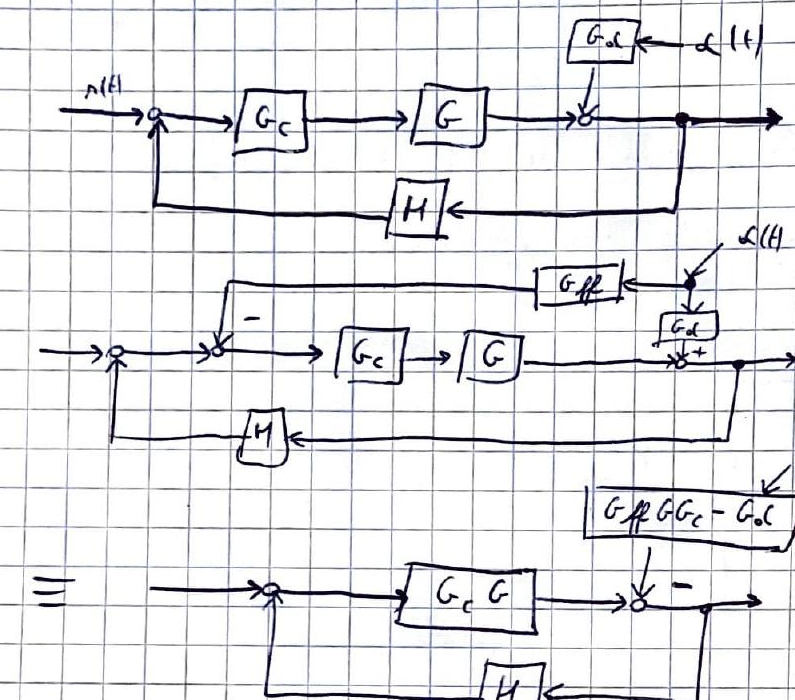
\includegraphics[width=.83\linewidth]{automatica_mod_1_tex_assets/b36_p46_1.png}\end{center}
\[
G_d=1\quad\Longrightarrow\quad d(t)=d_2(t),\qquad
G_d=G\quad\Longrightarrow\quad d(t)=d_1(t).
\]
Progetto controllori che provano ad annullare $d(t)$ prima che intervenga sul ramo diretto.
Per annullare il disturbo:
\[
G_{\mathrm{ff}}GG_c-G_d=0
\quad\Longrightarrow\quad G_{\mathrm{ff}}=\frac{G_d}{GG_c}.
\]
Ma probabilmente $GG_c$ ha il denominatore di grado maggiore di quello di $G_d$, quindi $G_{\mathrm{ff}}$ sarebbe impropria (e quindi irrealizzabile).
\paragraph{Esempio}
\[
G_d=\frac1{s+p},\qquad G_cG(s)=\frac{\omega_n^2}{s^2+2\delta\omega_ns+\omega_n^2},
\]
\[
G_{\mathrm{ff}}=\frac{s^2+2\delta\omega_ns+\omega_n^2}{(s+p)\omega_n^2},
\qquad m=2,\quad n=1,\quad m>n:\ \text{impropria}.
\]
% Pagina originale 47
\pagina{47}
\subsection*{Sensibilità alle variazioni parametriche}
\begin{center}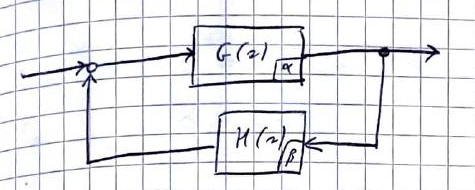
\includegraphics[width=.67\linewidth]{automatica_mod_1_tex_assets/b36_p47_1.png}\end{center}
\[
G(s;\alpha),\qquad H(s;\beta).
\]
Suppongo che il parametro abbia una certa precisione:
\[
\alpha=\underbrace{\alpha_0}_{\text{valore nominale}}
+\underbrace{\Delta\alpha}_{\text{variazione parametrica}}.
\]
Si dice sensibilità di $G(s)$ rispetto ad $\alpha$ la funzione
\[
S_\alpha^G\mathrel{\triangleq}\lim_{\Delta\alpha\to0}
\frac{\Delta G/G}{\Delta\alpha/\alpha}
=\frac{\partial G}{\partial\alpha}\frac\alpha G.
\]
\paragraph{Esempio}
\[
G(s;\alpha)=\frac1{s+\alpha}.
\]
\begin{align*}
S_\alpha^G&=\frac{\partial G}{\partial\alpha}\frac\alpha G
=-\frac1{(s+\alpha)^2}\frac\alpha G\\
&=-\frac1{(s+\alpha)^2}\frac{\alpha(s+\alpha)}1
=-\frac\alpha{s+\alpha}.
\end{align*}
\subsection*{Regola della catena}
\[
S_\alpha^\beta=S_\alpha^\delta S_\delta^\beta.
\]
\[
G(s;\alpha)\simeq G(s;\alpha_0)+\Delta G(s)
=G(s;\alpha_0)+\left.\frac{\partial G}{\partial\alpha}\right|_{\alpha=\alpha_0}\Delta\alpha.
\]
\subsection*{Luogo delle radici}
\begin{center}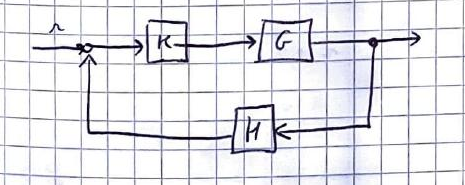
\includegraphics[width=.65\linewidth]{automatica_mod_1_tex_assets/b36_p47_2.png}\end{center}
\[
G_0(s)=\frac{kG(s)}{1+kG(s)H(s)}.
\]
Studiamo l'equazione caratteristica, $a_0=1+kGH=0$.
Si chiama luogo delle radici il luogo dei punti del piano complesso che risolvono l'equazione caratteristica
\[
1+kGH=1+kL(s)=0
\]
per tutti i valori positivi di $k$ ($k\in\mathbb R^+$).
% Pagina originale 48
\pagina{48}
Il luogo dei punti che risolvono l'equazione caratteristica con $k\in\mathbb R^-$ è chiamato luogo delle radici complementare.
\[
\overline s\in\mathrm{LdR}_+\quad\Longrightarrow\quad
\exists\overline k\in\mathbb R^+:a_0(\overline s)=0,
\]
\[
\overline s\in\mathrm{LdR}_-\quad\Longrightarrow\quad
\exists\overline k\in\mathbb R^-:a_0(\overline s)=0.
\]
Considero
\[
a_0(s)=1+kL(s)=0\quad\Longrightarrow\quad L(s)=-\frac1k
\quad\Longleftrightarrow\quad
\begin{cases}|L(s)|=|1/k|&\text{equazione di taratura},\\
\arg L(s)=\arg(-1/k)&\text{regola delle fasi}.\end{cases}
\]
\[
\arg L(s)=\arg\left(-\frac1k\right).
\]
\subsection*{Regola delle fasi}
\[
\arg L(s)=\arg\left(-\frac1k\right)
\quad\Longrightarrow\quad
\arg L(s)=\begin{cases}(2\nu+1)\pi&k>0,\\2\nu\pi&k<0.\end{cases}
\]
\begin{align*}
\arg L(s)&=\arg\frac{\prod_i(s-z_i)}{\prod_i(s-p_i)}
=\sum_i\arg(s-z_i)-\sum_i\arg(s-p_i)\\
&=\sum_{i=1}^{m}\varphi_i-\sum_{i=1}^{n}\theta_i
=\begin{cases}(2\nu+1)\pi&k>0,\ \mathrm{LdR}_+,\\
2\nu\pi&k<0,\ \mathrm{LdR}_-.\end{cases}
\end{align*}
Con $\varphi_i=\arg(s-z_i)$ e $\theta_i=\arg(s-p_i)$.
\paragraph{Esempio}
\[
L(s)=\frac{s+1}{s(s+2)},\qquad
\arg L(s)=\arg(s+1)-\arg s-\arg(s+2)
=\begin{cases}(2\nu+1)\pi&k>0,\\2\nu\pi&k<0.\end{cases}
\]
\[
\overline s=-1+j,\qquad
\overline s+1=\overline s-z_1,\quad
\overline s=\overline s-p_1,\quad
\overline s+2=\overline s-p_2,
\]
\[
z_1=-1,\qquad p_1=0,\qquad p_2=-2.
\]
\[
\arg L(\overline s)=\arg j-\arg(-1+j)-\arg(1+j)
=\frac\pi2-\frac{3\pi}4-\frac\pi4=-\frac\pi2.
\]
% Nota conclusiva manoscritta alla fine della pagina 48 non chiaramente leggibile; il calcolo è interamente trascritto.
% Pagina originale 49
\pagina{49}
\[
-\frac\pi4\ne(2\nu+1)\pi\quad\land\quad-\frac\pi4\ne2\nu\pi
\quad\Longrightarrow\quad
\overline s\notin\mathrm{LdR}_+\quad\land\quad\overline s\notin\mathrm{LdR}_-.
\]
% La pagina precedente calcola -pi/2; qui il manoscritto scrive -pi/4. Entrambi conservati.
La regola delle fasi rappresenta una verifica, non un modo per trovare le radici.
\subsection*{Equazione di taratura}
\[
|k|=\frac1{|L(s)|}=\frac{\prod_i\rho_i}{\prod_i\chi_i},
\qquad\rho_i=|s-p_i|,\quad\chi_i=|s-z_i|.
\]
$k$ aumenta allontanandosi dai poli e avvicinandosi agli zeri.
\subsection*{Regole di Evans}
\begin{enumerate}
\item Il luogo delle radici è sempre simmetrico rispetto all'asse reale.
\item Il luogo delle radici ha numero di rami pari al numero dei poli di $L(s)$.
\item Ogni polo dà origine ad un ramo ($k\to0$) che o confluisce in uno zero o diverge. Ci sono $n-m$ asintoti ad un ramo all'infinito ($n$ è il numero dei poli, $m$ il numero degli zeri).
\end{enumerate}
\begin{center}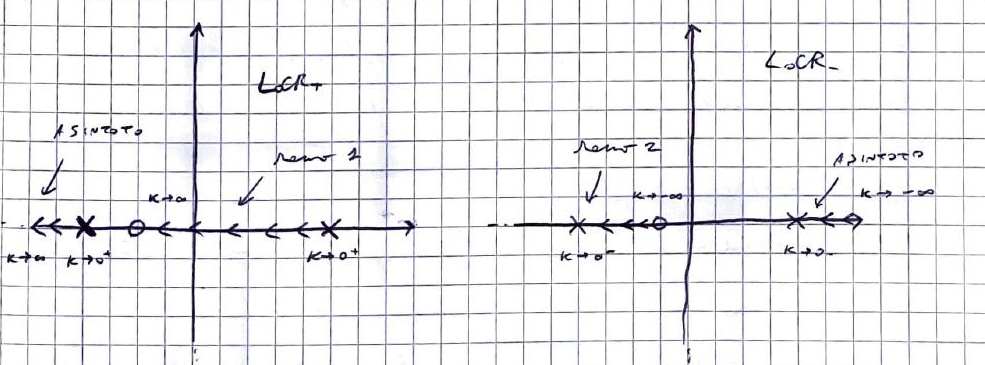
\includegraphics[width=\linewidth]{automatica_mod_1_tex_assets/b36_p49_1.png}\end{center}
\[
\lim_{s\to p}|L(s)|=\infty\quad\Longrightarrow\quad|k|\to0,
\qquad
\lim_{s\to z}|L(s)|=0\quad\Longrightarrow\quad|k|\to\infty.
\]
% Pagina originale 50
\pagina{50}
\begin{enumerate}\setcounter{enumi}{3}
\item Un punto $s\in\mathbb R$ appartiene a $\mathrm{LdR}_+$ [$\mathrm{LdR}_-$] se alla sua destra ci sono un numero dispari [pari] di poli o zeri.
\end{enumerate}
La dimostrazione viene dalla regola delle fasi.
In $\mathrm{LdR}_+$:
\[
\arg L(\overline s)=(2\nu+1)\pi.
\]
Le fasi per le coppie complesse di poli si annullano. Per ogni polo sottraggo $\pi$, per ogni zero aggiungo $\pi$:
\[
m\pi-n\pi=(m-n)\pi,
\qquad m-n\text{ dispari}=2\nu+1.
\]
Per $\mathrm{LdR}_-$, $\arg L(s)=2\nu\pi$, quindi il numero di poli e di zeri devono essere pari.
\begin{enumerate}\setcounter{enumi}{4}
\item I rami che tendono all'infinito si ritrovano tutti in un punto dell'asse reale $\sigma$, detto centroide:
\[
\sigma=\frac{\sum_i^np_i-\sum_i^mz_i}{n-m}.
\]
Gli angoli degli asintoti si calcolano come
\[
\theta_{a,\nu}=\begin{cases}
\frac{(2\nu+1)\pi}{n-m}&k>0,\ \mathrm{LdR}_+,\\
\frac{2\nu\pi}{n-m}&k<0,\ \mathrm{LdR}_-,
\end{cases}\qquad \nu\in\mathbb N.
\]
\item Ci sono punti di confluenza e punti di emersione che sono le radici multiple di $a_0(s)=1+kL(s)=0$.
Si trovano risolvendo
\[
a'(s)b(s)-a(s)b'(s)=0,\qquad L(s)=\frac{b(s)}{a(s)}.
\]
I punti di confluenza sono i punti dell'asse reale nei quali confluiscono due o più rami.
I punti di emersione sono i punti dell'asse reale dai quali emergono due o più rami.
\end{enumerate}
% Pagina originale 51
\pagina{51}
\begin{enumerate}\setcounter{enumi}{6}
\item Angolo di partenza di un ramo da un polo:
\[
\theta_{p,\nu}=\frac1r\left[
\sum_i\arg(p-z_i)-\sum_{p_i\ne p}\arg(p-p_i)
+\begin{cases}(2\nu+1)\pi&k>0,\\2\nu\pi&k<0\end{cases}\right].
\]
$r$: molteplicità.
\begin{center}
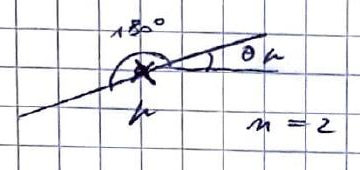
\includegraphics[width=.45\linewidth]{automatica_mod_1_tex_assets/b36_p51_1.png}\quad
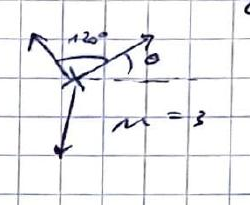
\includegraphics[width=.32\linewidth]{automatica_mod_1_tex_assets/b36_p51_2.png}
\end{center}
Molteplicità $r=2$: angoli separati di $180^\circ$; $r=3$: angoli separati di $120^\circ$.
\item Angolo di arrivo agli zeri:
\[
\theta_{z,\nu}=\frac1r\left[
\sum_i\arg(z-p_i)-\sum_{z_i\ne z}\arg(z-z_i)
+\begin{cases}(2\nu+1)\pi&k>0,\\2\nu\pi&k<0\end{cases}\right].
\]
\item Il luogo delle radici interseca l'asse immaginario per valori di $k$ che annullano una riga dispari della tabella di Routh.
\end{enumerate}

\end{document}
